\documentclass[12pt]{article} 

\usepackage{amsfonts,amsmath,amssymb,amsthm}
\usepackage{array}
\usepackage{authblk}
\usepackage{color}
\usepackage[table]{xcolor}
\usepackage{epsfig,fancyhdr}
\usepackage{geometry,graphicx}
\usepackage[]{hyperref} 
\usepackage{indentfirst}
\usepackage{mathtools}
\usepackage{multirow}
\usepackage{listings}
\usepackage{natbib}
\usepackage{rotating}
\usepackage{comment}
\usepackage{booktabs}
\usepackage{todonotes}
\setuptodonotes{inline}
\usepackage{makecell}
\usepackage{enumitem}
\usepackage{tcolorbox}

%%%%%%%%%%%%%%%%%%%%%%%%%%%%%%%%%%%%%%%%%%%%%%%%%%%%%%%%%%%%%%%%%%%%%%%%%%%%%%%%%%%%%%%%
\usepackage{sectsty,secdot}
\sectionfont{\bf\fontsize{14}{2em}\selectfont}
\subsectionfont{\bf\fontsize{12}{2em}\selectfont}
%%%%%%%%%%%%%%%%%%%%%%%%%%%%%%%%%%%%%%%%%%%%%%%%%%%%%%%%%%%%%%%%%%%%%%%%%%%%%%%%%%%%%%%%

\geometry{left=2.5cm,right=2cm,top=2.5cm,bottom=1.5cm}
\setlength{\parindent}{0.63cm}

\setcounter{page}{1}
\newtheorem{theorem}{Theorem}
\newtheorem{lemma}{Lemma}
\newtheorem{corollary}{Corollary}
\newtheorem{proposition}{Proposition}
\theoremstyle{definition}
\newtheorem{definition}{Definition}
\newtheorem{example}{Example}
\newtheorem{remark}{Remark}
\pagestyle{empty}
\usepackage{lineno}
\setcitestyle{square}

\newcommand*\rot{\rotatebox{90}}

%---------page header---------%

%\fancyhead[RO]{odd number page}
%\fancyhead[LE]{even number page}

\pagestyle{plain} 
\linenumbers

%-----------------------------%
\newtheorem{question}{Question}

\newtheorem{requirement}{Requirement}


\renewcommand{\_}{%
    \textunderscore\hspace{0pt}%
}
\setlength{\emergencystretch}{3em}

\newtcolorbox{redbox}{colback=red!5!white,colframe=red!75!black,width=3cm}
\newtcolorbox{yellowbox}{colback=yellow!5!white,colframe=yelloe!75!black,width=3cm}


\newcommand{\DONE}{{\color{green!60!black}\makebox[0pt][l]{$\square$}\raisebox{.15ex}{\hspace{0.1em}$\checkmark$}}~}
\newcommand{\DOIT}{{\color{red!60!black}\makebox[0pt][l]{$\square$}\raisebox{.15ex}{\hspace{0.1em}$\boxtimes$}}~}
\newcommand{\PROGRESS}{(in progress)~}

\begin{document}

\input{response-2-content}

\title{{\bf\fontsize{14pt}{18pt}\selectfont AICov: An Integrative Deep Learning Framework for COVID-19 Forecasting with Population Covariates}}
\author[1]{{\fontsize{12pt}{0.5em}\selectfont Geoffrey C. Fox}}
\author[1]{{\fontsize{12pt}{18pt}\selectfont Gregor von Laszewski}}
\author[1]{{\fontsize{12pt}{0.5em}\selectfont Fugang Wang}}
\author[2,3]{{\fontsize{12pt}{0.5em}\selectfont Saumyadipta Pyne}}

\affil[1]{{\fontsize{12pt}{0.5em}\selectfont Digital Science Center, Indiana University, Bloomington Indiana, USA}}
\affil[2]{{\fontsize{12pt}{0.5em}\selectfont Public Health Dynamics Lab, and Department of Biostatistics, University of Pittsburgh, Pittsburgh, Pennsylvania, USA}}
\affil[3]{{\fontsize{12pt}{0.5em}\selectfont Health Analytics Network, Pennsylvania, USA}}

\newcommand{\ABSTRACT}{
The COVID-19 pandemic has had profound global consequences on health, economic, social, behavioral, and almost every major aspect of human life. Therefore, it is of great importance to model COVID-19 and other pandemics in terms of the broader social contexts in which they take place. 
We present the architecture of an artificial intelligence enhanced COVID-19 analysis (in short AICov) , which provides an integrative deep learning framework for COVID-19 forecasting with population covariates, some of which may serve as putative risk factors. 
We have integrated multiple different strategies into AICov, including the ability to use deep learning strategies based on LSTM and event modeling.
To demonstrate our approach, we have introduced a framework that integrates population covariates from multiple sources. Thus, AICov not only includes data on COVID-19 cases and deaths but, more importantly, the population's socioeconomic, health, and behavioral risk factors at a local level. The compiled data are fed into AICov, and thus we obtain improved prediction by the integration of the data to our model as compared to one that only uses case and death data. As we use deep learning our models adapt over time while learning the model from past data.
}
\date{}
 
\newcommand{\TODO}[1]{
\todo[color=yellow!20]{#1}
}


%%%%%%%%%%%%%%%%%%%%%%%%%%%%%%%%%%%%%%%%%%%%%%%%%%%%
\renewcommand{\baselinestretch}{1.07}
\renewcommand{\thefootnote}{}
%%%%%%%%%%%%%%%%%%%%%%%%%%%%%%%%%%%%%%%%%%%%%%%%%%%%


\maketitle
\thispagestyle{empty}

\begin{quotation}
\centerline{\bfseries{\fontsize{14pt}{1em}\selectfont Abstract}}\par
\setlength{\parindent}{3.22cm}
{\fontsize{12pt}{1.07em}\selectfont~~\ABSTRACT}

\vspace{12pt}
\noindent {\bfseries{Key words and phrases:}}
COVID-19, deep learning, prediction, risk factors, comorbidities.
\par
\end{quotation}\par

\def\thefigure{\arabic{figure}}
\def\thetable{\arabic{table}}

\renewcommand{\theequation}{\thesection.\arabic{equation}}

\fontsize{12}{1.07em}\selectfont

\setcounter{section}{0} %***
\setcounter{equation}{0} %-1


\section{Introduction}

The COVID-19 pandemic has caused an enormous health and humanitarian crisis worldwide. It is unlike any other single phenomenon that has occurred in modern history since the end of World War II. 
The pandemic’s effects have spanned over a range that is so vast over space, and yet so condensed over time, that the dual blows of intensity and rapidity have exposed myriad systemic vulnerabilities in many societies around the world. 

The first known case was traced back to  17  November  2019. Since the emergence of a cluster of cases in Wuhan, China, on 31 December 2019, COVID-19 has spread rapidly worldwide. Just six months later, as of 23 June 2020, there are 8,993,659 COVID-19 cases and 469,587 deaths globally. On 30 January 2020, the World Health Organization (WHO) \cite{www-who} declared COVID-19 to be a Public Health Emergency of International Concern and subsequently, on 11 March 2020, a pandemic.

In the United States, the first case of COVID-19 was confirmed on 20 January 2020 in Washington State, and as of 23 June 2020, there were over 2.3 million confirmed cases and 121,167 deaths \cite{www-nyt-map}. 
Although initial efforts to reduce the spread took place, recent data shows a resurgence at an increased scale. In the absence of a vaccine or treatment to effectively combat the disease, non-pharmaceutical policy interventions such as social distancing and lockdowns are recommended by health experts to prevent further transmission. To gain insights into the possible impact of such measures on COVID-19 outcomes, we depend upon the ability to accurately forecast the spread of reported cases and confirmed deaths and recoveries. Naturally, the accuracy of forecasting relies on the availability of current, reliable data and historical data to determine estimates of uncertainty.

During outbreaks of epidemics, initially data on cases and deaths could be scarce, and the quality of data annotation, validation, and aggregation might be uncertain. For instance, changes in clinical data entry, such as the addition of a new category clinically diagnosed to the existing lab-confirmed category, may likely have been reflected in the reporting \cite{Petropoulos2020-hh}. Initial fears about COVID-19 among the general population with regards to the trajectory of the pandemic could also affect administrative reporting. Diverse media sources and differences in local and federal policies may add to the general uncertainty about disease progression. Nevertheless, a data-driven approach to forecasting can offer valuable insights into the disease dynamics, and thereby an ability to objectively plan for the near future. 

Unlike earlier global outbreaks, during COVID-19, the current worldwide digital ecosystem allows for real-time data collection, which in turn is used by artificial intelligence (AI) and deep learning systems to understand healthcare trends, model risk associations, and predict outcomes \cite{Ting2020-lw}. 
In addition to traditional public health surveillance strategies available to most countries, a variety of static and dynamic data types may be integrated to model the scale and dynamics of this pandemic \cite{Pyne2015-ao}. Several organizations, including the Johns Hopkins University’s Center for Systems Science and Engineering, the New York Times, the Atlantic’s COVID-19 tracking project, among others have developed real-time tracking maps for following COVID-19 cases around the world using data from the U.S.~Centers for Disease Control and Prevention (CDC), WHO, and other international health agencies. Notably, the CDC receives forecasts from several modeling groups that use a wide variety of approaches ranging from SEIR (Susceptible-Exposed-Infectious-Recovered) to Agent-based to Bayesian models to understand the non-pharmaceutical policy interventions (or the lack thereof) to predict disease dynamics and its impact on human lives \cite{www-cdc-modeling-forecast}.

For precise and contextually relevant modeling of COVID-19 dynamics for a given population or community, we use data integration to combine community-specific health and behavioral risk factors, demographic and socioeconomic variables that are available at the local levels along with the cases and deaths data for COVID-19 while leveraging the recently developed and increasingly popular deep learning strategies to forecast COVID-19 dynamics using our model. Towards this, we develop a parallel computing platform called AICov standing for  AI-driven Platform for COVID-19 to implement the different components of our framework and obtain the needed resources through multi-cloud interfaces in a robust manner. 

In this study, while we incorporate information from community and county-specific covariates to inform our forecasting model for each metropolitan area, we want to avoid the so-called ecological fallacy in drawing inferences about individual disease outcomes based on large area-level aggregated risk factors. Our objective is also to underscore the nuanced roles played by pre-existing socioeconomic and other prevailing conditions of a given community that can act as determinants of its health outcomes and possible disparities,  especially under such sudden stresses to its current systems as those felt during any pandemic.
It is important to note that the underlying models are learned directly from the data instead of being projected by a theoretical epidemiological model that relies on simulation populations. This allows quick adaptation and self-adaptation in regards to changing behaviors and regional differences. 

The paper is structured as follows. In Section \ref{sec:lstm-theory}, we provide a short overview of deep learning-based time series forecasting that we use in AICov. In Section \ref{sec:arch}, we outline our architecture that enables the user to conduct powerful time series forecasting by integrating static and dynamic information on population risk factors with time-series disease data. In Section \ref{sec:data}, we describe the input data for AICov. Next, we demonstrate our analysis involving the population risk factors and identify those that contribute to our prediction accuracy. Finally, we present our conclusion.



\section{LSTM}
\label{sec:lstm-theory}

This section presents a short overview of the recurrent neural network algorithms used in this work.


% ------------------------------
\subsection{LSTM Background}
\label{sec:lstm-background}
% ------------------------------

In this study, we used a Long Short-Term Memory (LSTM) algorithm for our predictions \cite{www-keras-lstm,Hochreiter1997-dk}. An LSTM is a recurrent neural network (RNN) \cite{Rumelhart1986-li} with feedback connections allowing the use of data input sequences to predict data output sequences. LSTMs have been applied to many application areas from handwriting \cite{Graves2009-qb}, image, feature detection, and time series prediction \cite{Schmidhuber2005-oy}. LSTM's have an internal state that is used to prevent the vanishing gradient problem \cite{Hochreiter1991-mp} during the training of RNNs.

Different variants of LSTM algorithms exist. Ours is based on an LSTM cell depicted in Figure \ref{fig:lstm}. 
It has an input gate, output gate, and a forget gate. The cell is maintaining how a subsequent value is calculated. This includes (a) how input values are influencing the cell via the input gate, (b) how the forget gate influences a memory value within the cell via the forget gate, and (c) how the output gate influences the output activation of the LSTM unit. A cell has a number of inputs and outputs that are weighted. During a training step, these weights are learned to be reused in a prediction process between input and output sequences.

\begin{figure}[h!]
\begin{minipage}[b]{0.6\textwidth}
    \centering
    \includegraphics[width=0.6\columnwidth]{images/lstm.pdf}
    \caption{LSTM Unit Diagram}
    \label{fig:lstm}
\end{minipage}
\ \
\begin{minipage}[b]{0.3\textwidth}
\vspace{-3cm}
\begin{equation*}
\begin{split}
    f_t &= \sigma(W_f x_t + U_f h_{t-1} + b_f) \\
    i_t &= \sigma(W_i x_t + U_i h_{t-1} + b_i) \\
    o_t &= \sigma(W_o x_t + U_o h_{t-1} + b_o)\\
    \tilde{c}_t &= tanh(W_c x_t + U_c h_{t-1} + b_c)\\
    c_t &= f_t \circ c_{t-1} +i_t \circ \tilde{c}_t \\ 
    h_t &= o_t \circ tanh(c_t) 
    \label{eq:lstm_equations}
\end{split}
\end{equation*}
\caption{LSTM Equations}
\label{fig:eq}
\end{minipage}
\end{figure}

\newcommand{\Rh}{\mathbb{R}^{h}}

We have summarized the equations used in LSTM in Figure~\ref{fig:eq}. We denote variables in lower case and matrices in upper case letters. $W_{q}$ and $U_{q}$ contain the weights of the input and recurrent connections, where the subscript denotes either the input gate $i$, the output gate $o$, the forget gate $f$ or the memory cell $c$.  It is important to note that  $c_{t}\in \mathbb {R}^{h}$ is not just one cell of one LSTM unit, but contains $h$ LSTM units' cells, representing a vector. To summarize our variables we use:
$\circ$ is the Hadamard product,
$\sigma$ is the sigmoid function,
$d$ the number of input features,
$h$ the number of hidden units,
$x_{t}\in \mathbb R^d$ the input vector to the LSTM unit,
$f_t\in \Rh$ the forget gate's activation vector,
$i_{t}\in \Rh$ the input/update gate's activation vector,
$o_{t}\in \Rh$ the output gate's activation vector,
$h_{t}\in \Rh$ the hidden state vector (e.g., the output vector of the LSTM unit),
$\tilde{c}_t\in \Rh$ the cell input activation vector,
$c_{t}\in \Rh$ the cell state vector,
$W\in \mathbb{R}^{h\times d}$, $U\in \mathbb{R} ^{h\times h}$, and $b\in \Rh$ are the weight matrices and bias vector parameters which need to be learned during training.


\subsection{Covariate Enhanced LSTM}

We often think of the laws of physics described by operators that
evolve the system given sufficient initial conditions and in this
language, we have shown how to represent Newton’s law operator by a
recurrent network \cite{Kadupitiya2020-zq}. We expect that the time
dependence of many complex systems: Covid pandemics, Southern
California earthquakes, traffic flow, security events can be described
by deep learning operators that both capture the dynamics and allow
predictions. 

In this paper, we adopt this approach to describe the
time dependence of COVID-19 infection and fatality counts in different
regions. 
We intend to
process the two time-series (infections, fatalities/deaths) associated with
each city plus the covariates (fixed in time but dependent on region)
to build a model for the time evolution of the data. There is a
nontrivial architecture design choice as to the method of handling the
time-independent covariates. We could combine a recurrent network for
the time series with some fixed network for the covariates. However,
that does not fit with our concept of deriving an evolution operator
for COVID-19 data that naturally depends on the covariates for each
city. Thus instead, we feed the covariates into the recurrent network.

\section{AICov Architecture}
\label{sec:arch}

The motivation for creating this architecture is based on our experience with deep learning toolkits such as Keras and PyTorch. While these systems provide the necessary APIs to integrate time series solutions, they target primarily more general user communities. In particular, they do not consider existing data sets or specific needs and analysis options to evaluate them for the purpose of COVID-19 risk factor data integration. We describe below the different requirements that motivate the design of our architecture framework, AICov, and how we address each of these.

%\newcommand{\Solution}{{\bf Solution: }}
\newcommand{\Solution}{}

\begin{requirement}{\bf Ease of Use.} A major design criterion for AICov is that the framework must be easy to use, and extensions can be made to allow usability of both the API as well as the user interface. \Solution To address these requirements, we are devising a specialized but easy to use time series API for COVID-19 that integrates common tasks such as automated filtering and normalization of the data.
\end{requirement}


\begin{requirement}{\bf Interactive Access.} Due to the experimental nature of analyzing the data, AICov must support the exploration of the data in an interactive fashion. \Solution As many data scientists use Jupyter Notebooks to integrate their work interactively, AICov integrates such notebooks. Jupyter notebooks allow rapid modification of the analysis workflow through the ease of Python as programming language. Additionally, they enable us to formulate easily sophisticated scientific analytics workflows with the help of Python.
\end{requirement}


\begin{requirement}{\bf Expandable API.} Assuming that new models and other analysis algorithms will be developed over time, AICov must allow the integration of such APIs. \Solution To address this requirement, we are developed an abstraction API for data, analysis, and metadata parameter adjustments. External services could be integrated with the help of REST (REpresentational State Transfer) services. The REST services are automatically generated from function specifications. 
\end{requirement}


\begin{requirement}{\bf Flexible Data Source Integration.} The integration of various sources of data is a key part of AICov. \Solution To achieve this goal, we provide a number of abstractions and data manipulation functions to extract needed data from established sources. Furthermore, the data can be combined, and additional data wrangling by external groups can be integrated.
Through such abstractions, it is possible to replace, add, and correct data sets that are part of the analysis. This allows us to compare different results created from different data sets. Moreover, we include data selection directly in our framework to easily and quickly reuse them in a data mashup. An important example is that the data need not be static over the disease's progression but can be continuously updated. This also has a significant impact on our analytics algorithms.
\end{requirement}

\begin{requirement}{\bf Automated Update of the Analytics.} As the data can change, previous analyses may have to be updated. \Solution Our forecast is not just a single script but includes a mechanism to register multiple workflows of continuously integrated (CI) analysis that are automatically rerun when new data are made available to the system. Previous results are maintained. Metadata with these runs can retrieve the versioned data sets used to calculate and store the versioned analytics workflow.
\end{requirement}

\begin{requirement}{\bf Flexible Model definition.} We want to allow experimentation with various models in AICov that may be easily and flexibly definable as workflows. \Solution We give functional abstraction definitions that enables us to define the models ourselves or integrate third party models describing the spread of the disease. 
\end{requirement}

\begin{requirement}{\bf Deep Learning Forecast.} As the forecasting models depend on changing data that are made available daily, it is important for AICov to utilize the newly available data. Many models can be applied to this, including moving averages based models or models that are purely derived from deep learning. \Solution To address this requirement, AICov allows for the integration of both. Furthermore, in our deep learning framework, we can  integrate an automated search for important risk factors, which is the focus of this study.
\end{requirement}

\begin{requirement}{\bf Model Orchestration.} To coordinate the different model predictions and the generation of the deep learning forecasts, we need the ability to orchestrate them while applying a number of parameters. \Solution To address this requirement, the AICov architecture includes the ability to integrate parameter sweeps to, for example, identify hyperparameters, or integrate different data sets as parameters to identify suitable forecast models that can deliver the one which fits the best.
\end{requirement}

\begin{requirement}{\bf Compute Resource Mapping.} For other uses of AICov, we need to integrate a flexible resource utilization framework. \Solution To address this requirement, we leverage from our earlier work and utilize through Cloudmesh and NIST NBDIF definitions cloud services into the architecture \cite{las-19-nist}. This includes containers but also infrastructure services in the cloud. Through these service integrations, we also provide access to  GPUs.
\end{requirement}

\begin{requirement}{\bf Convenient Interfaces.} As we have a wide variety of users, we need to enable interfaces that are used by the various communities. \Solution To address this requirement, we provide a number of APIs, REST services and make them available via Jupyter Notebooks. In addition, we developed some custom widgets for the notebooks that are specifically targeted towards data integration, parameter manipulation, and visualization of the results 
\end{requirement}


Putting all these requirements together results in an architecture as shown in Figure \ref{fig:arch}.\\

\begin{figure}[h!]
    \centering
    \includegraphics[width=0.6\columnwidth]{images/arch.pdf}
    \caption{AICov Architecture}
    \label{fig:arch}
\end{figure}

In summary, the AICov architecture allows the inclusion of new data sources and models. An orchestrator enables modifying parameters and selecting data sources and models used in the analysis. The framework can be accessed via the interface layer that includes APIs, REST, and Jupyter Notebooks. Compute interfaces are provided either by direct access of GPUs from local resources or through the staging of automatically generated REST services via our Cloudmesh REST Service integrator \cite{cloudmesh-openapi-install,cloudmesh-openapi-benchmark,cloudmesh-manual}. Additionally, we can also access through abstractions cloud services that are offered by the various cloud providers and are targeting our application domain. Different models can be easily integrated into our framework to verify our forecast or enhance our forecast based on the users' models and data.

\section{Data for the COVID-19 Analysis}
\label{sec:data}

While the U.S. has seen an overall case fatality rate of 5.14\%, 
some U.S. locations have experienced a disproportionate number of deaths compared to others. This disparity of deaths among different communities could be attributed to a diversity of local risk factors and socioeconomic determinants of health that now constitute a very active area of investigation. Researchers are studying the effects of different community-specific socioeconomic variables, underlying health conditions and comorbidities, infrastructure, and systemic responses.
Given the complexity of such underlying conditions that can determine individual disease outcomes,  where and under what conditions people get infected by the virus, and then recover or die take place not in isolation but rather in an interplay of diverse factors that are characteristic to a local community, which need to be synthesized. In other words, a basic requirement for effective modeling of COVID-19 dynamics is that the information regarding a particular community’s vulnerabilities and strengths pertaining to the disease must be as comprehensive and integrative as possible. 
The regular reporting of accurate Coronavirus outbreaks data from local health departments has been understandably difficult, especially in the areas that are hardest hit. We use data on community-specific health and behavioral risk factors aggregated at the county level from the large-scale longitudinal CDC BRFSS surveys \cite{www-cdc-brfss}, and demographic and socioeconomic data from the U.S. Census Bureau that are known at the local levels along with the cases and deaths data compiled by NCHS \cite{www-cdc-nchs} and integrate them with other data sources.

\subsection{Data Collection and Processing}

Among the different sources of data on daily cases and deaths data collected and aggregated at different spatial levels, especially for the U.S., many are either freely available repositories such as GitHub or accessible via specifically developed online resources such as the New York Times~\cite{github-nytimes} and the Johns Hopkins Coronavirus Resource Center~\cite{www-jh-covid19}. 
For this study, we generated two data sets based on the latter resource upon our checking for the locations and times at which cumulative counts of COVID-19 cases and deaths on any given day were no less than those on the previous day. This led us to compile daily coronavirus cases and deaths data for 345 U.S. counties from 32 states and the District of Columbia and matched by five-digit FIPS code or county name to dynamic and static variables from additional data sources.

The static data in this repository was collected from the U.S. Census Bureau and the Centers for Disease Control and Prevention (CDC). The different fields cover the domains of behavioral and health risk factors, hospital capacity, and socioeconomic and demographic conditions. Data on health outcomes, prevention measures, and unhealthy behaviors were extracted from the CDC's 500 Cities Local Data for Better Health program \cite{www-cdc-chronic-data} in the form of crude or age-adjusted prevalence of conditions such as respiratory disease, obesity or smoking. These values were aggregated from the census tract to the county level using the first five digits of the eleven-digit tract FIPS code. Because a single county may consist of multiple individual cities, we include the list of all city labels within each aggregate group to represent a greater metropolitan area. 110 of such metropolitan areas that had more than 500 reported cases of COVID-19 by April 15, 2020, were selected for this study.

Notably, a greater metropolitan area such as New York City could be spread across more than one county, which can lead to the complexity of aggregating counts and other variables. Time series data for the 5 individual counties (boroughs) in New York City were not available in the Johns Hopkins CSSE (Center for Systems Science and Engineering) data set. Rather, the total number of cases and deaths for the entire city of New York are reported and assigned the FIPS code of New York County (Manhattan). To ensure consistent geography across the static and dynamic data, we compute the population-weighted sum or median of each covariate over the assigned counties.

Demographic variables were gathered from the Census QuickFacts~\cite{www-census} online resource using an automated web scraping algorithm and cover relevant areas such as age, race, income, and population density. Additional socioeconomic variables include the Gini Index, which measures economic inequality and CDC Social Vulnerability Index (SVI)~\cite{www-cdc-svi}. The SVI was created to guide public health officials and disaster response efforts by identifying the communities across the United States most likely to need support during a crisis. Census tracts and corresponding counties are ranked across 15 social factors, which are grouped into four themes: socioeconomic status, household composition and disability, minority status and language, and housing and transportation.

Lastly, the total number of general acute care, critical access, and military hospitals within each county are included in the data. Such variables included the number of relevant hospitals per county, and the estimated number of beds (total known bed counts added to the number of hospitals in the county with missing data times the average number of beds per hospital in that state) per 1,000 people using the American Hospital Directory~\cite{www-ahd}.

The list of covariates is presented in Table \ref{tab:risk-factors}.


\begin{table}[!hptb]
\caption{Covariate Risk factor abbreviations as used in this study.}
\label{tab:risk-factors}
\bigskip
\resizebox{0.90\textwidth}{!}{
\centering
\begin{tabular}{ll}
\toprule
Risk Factor & Description \\
\midrule
 NONE & No risk factor used\\
 ARTHRITIS 	  & Percent reported with arthritis \\
 BINGE 		  & Percent reported with binge drinking \\
 BPHIGH 	  & Percent reported with  high blood pressure\\
 BPMED 		  & Percent reported taking blood pressure medication\\
 CANCER 	  & Percent reported as cancer patients\\
 CASTHMA 	  & Percent reported with current asthma\\
 CHD 		  & Percent reported with coronary heart disease\\
 CHECKUP 	  & Percent reported with health checkup\\
 CHOLSCREEN   & Percent reported with cholesterol screening\\
 COPD 		  & Percent reported with chronic obstructive pulmonary disease\\
 CSMOKING 	  & Percent reported as currently smoking\\
 DIABETES 	  & Percent reported with diabetes\\
 ESTBEDS 	  & Number of estimated beds in hospitals\\
 HIGHCHOL 	  & Percent reported with high cholesterol\\
 INSURANCE 	  & Percent reported with insurance\\
 KIDNEY 	  & Percent reported with kidney disease\\
 LPA 		  & Percent reported with no leisure-time physical activity \\
 MHLTH 		  & Percent reported with not good mental health\\
 NBEDS 		  & Number of beds in hospitals \\
 NBEDS/1000   & Number of beds per 1000 people\\
 NHOSP 		  & Number of hospitals\\
 OBESITY 	  & Percent reported with  population that is obese\\
 PHLTH        & Percent reported with physical health issues\\
 PVI 		  & Pandemic vulnerability index \\
 PERCENTBLACKS 	  & Percent of blacks in the population\\
 PERCENTHISPANICS & Percent of hispanics in the population\\
 STROKE 	  & Percent reported with stroke\\
 BLACK	  & Percent of Blacks in the population\\
 POVERTY & Percent of poverty in the population\\
 SENIOR  & Percent of seniors in the population\\
 SVI\_MINORITY 	  & Percent of social vulnerability index in the minority population\\
 SVI\_OVERALL 	  & Percent of social vulnerability index in the overall population\\
\bottomrule
\end{tabular}
}
\end{table}


\section{Analysis}

We have conducted a number of analysis efforts to evaluate the validity of our approach. We focus on the following questions:

\begin{question} Can we apply deep learning strategies that self-learn the behavior of a model in order to provide future predictions? See Section \ref{sec:emperical}.
\label{q:1}
\end{question}

\begin{question} Can we use real time data as input and apply deep learning strategies instead of models that self learn and provide future predictions? See Section \ref{sec:lstm-covariate}.
\label{q:2}
\end{question}

\begin{question} Does the inclusion of covariates improve the prediction quality while including geospatial and socio-economic risk factors? See Section \ref{sec:lstm-covariate}.
\label{q:3}
\end{question}

\begin{question} What impact do we see when we introduce many risk factors? See Section \ref{sec:lstm-many}.
\label{q:4}
\end{question}




\subsection{Deep Learning Predictions of Model-based Empirical Fits} 
\label{sec:emperical}

To establish the feasibility of using deep learning, we have, in our analysis, verified that through deep learning we can recreate the predictions identified by a model-based approach using empirical fits. In this comprehensive analysis, we obtain predictions through deep learning while using data generated from epidemiological models as discussed in \cite{marsland20-covid-paper}. The time series we used was 100 days long, and a multi-layered Long Short-Term Memory (LSTM) recurrent network was used. Our prediction approach differs by learning not only from the demographics (fixed data for each city) and time-dependent data but by integrating the population model for the underlying prediction, as shown in Fig. \ref{fig:magic-1}. Such model predictive integration capability is important in any application with multiple time scales. For example, this allows us to integrate multi-scale time effects into the forecast, which could address the combination of general forecasts and the next time steps of choice, such as days, weeks, months, or longer. For this analysis, we used 37 of the 110 cities with reliable empirical fits (that we derived from an epidemiological model and not deep learning  \cite{marsland20-covid-paper}) for the cases and deaths data up to April 15, 2020. Our analysis identified a sophisticated single deep learning time evolution operator that can describe these 37  separate data sets, and smooth fitted data leads to very accurate deep learning descriptions via LSTM as depicted in both Figure \ref{fig:magic-1} that are smaller than 1\% from the model predictions.



\begin{figure}[!h]
    \centering
    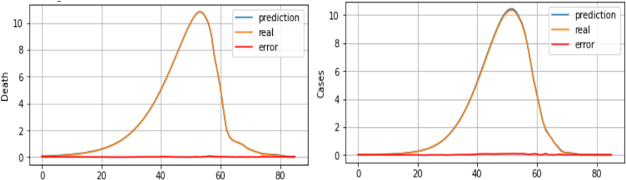
\includegraphics{images/magic-1.png}
    \caption{Cumulative empirical fits can be very accurately predicted with LSTM. The data is taken from 37 U.S. Cities. Our comparison showcases that given a model, we can replicate the prediction of such models using the model data over time. The x-axis represents the days since the first data was fed to the model.}
    \label{fig:magic-1}
\end{figure}




\subsection{Real time-Data Covariate LSTM Prediction}
\label{sec:lstm-covariate}

In this  section, we establish that using deep learning can not only be applied to model predictions from  real time data. As we want to evaluate the influence of the risk factors on our prediction framework using not only models but deep learning algorithms, we have devised a parameter sweep framework based on LSTM that conducts the prediction for the 110 cities while also considering the risk factors as listed in Table \ref{tab:risk-factors}. This framework can query any combination of risk factors as well as not including any, in which case it defaults to the traditional LSTM algorithm as introduced in Section \ref{sec:lstm-theory}. Hence, we will answer Questions \ref{q:2} and \ref{q:3}. 

To answer these questions, we chose for our next analysis a date range between 2020-02-01 and 2020-05-25. We start with a basic LSTM operator with two layers of LSTM, and initial and final fully connected layers \cite{Kadupitiya2020-zq}. 
For LSTM, we have selected the activation function based on Rectified Linear Units (RELU). For the last layer sigmoid is chosen. A drop out rate of 0.2 is used, we use 16 input nodes, and have a batch size of 110. The maximum epoch is chosen to be 200. The number of nodes internally is 32. The maximum total number of Samples is 12540 when using 3 days as input length. We use a two-layer LSTM, as shown in Table \ref{tab:model}. Within our system, we have the ability to set a number of input days. For this analysis, we have chosen three different input lengths, namely 3, 4, and 5 days. 


\begin{table}[!h]
    \caption{The deep learning parameters used for the model sweep creation in as exported by Keras using 1 risk factor. The activation function is RELU and the recurrent activation function is sigmoid.}
    \label{tab:model}
    \bigskip

    \settowidth{\rotheadsize}{Parameters\quad}

    \begin{footnotesize}
    \centering
    \resizebox{1.0\textwidth}{!}{ 
    \begin{tabular}{|ll|lll|ll|ll|}
    \toprule 
     \rothead{Layer} & \rothead{Type}   &
     \rothead{Output Shape} &  \rothead{Parameters for 0 risk factor}  
                  &  \rothead{Parameters for 1 risk factor} &
     \rothead{Output Shape} &  \rothead{Parameters for 33 risk factors} &
     \rothead{Output Shape} &  \rothead{Parameters for 37 risk factors}\\
    \midrule
    dense & Dense    & (None,1,32) & 96   & 128  &  (None,5,32) & 1152 & (None,5,32) & 1280 \\
    LSTM & LSTM      & (None,1,16) & 3136 & 3136 &  (None,5,16) & 3136 & (None,5,16) & 3136 \\
    LSTM 1 & LSTM   & (None,16)  & 2112  & 2112 &  (None,16)   & 2112 & (None,16)   & 2112 \\
    Dense 1 & Dense & (None,32)  &  544  & 544  &  (None,32)   &  544 & (None,32)   &  544 \\
    Dense 2 & Dense & (None,30)  &  990  & 990  &  (None,30)   &  990 & (None,30)   &  990 \\
    \bottomrule
    \end{tabular}
    }
    ~\\
    The LSTM contains a total of 6,910 trainable parameters in case we include one risk factor. In the case, we do not use any risk factor it is 6878, and when we include 33 risk factors, it is 7934.  
    \end{footnotesize}
\end{table}


\begin{comment}
\begin{verbatim}
    model.add(Dense(InitialMLP, activation=activationvalue, input_shape=(n_timesteps, n_features)))
        
    model.add(LSTM(n_nodes, unroll=True, recurrent_dropout= recurrent_dropout1, dropout = dropout1,
                   activation= activationvalue , return_sequences=True, recurrent_activation="sigmoid",
                   input_shape=(n_timesteps, nextround)))
                   
    model.add(LSTM(n_nodes, unroll=True, recurrent_dropout= recurrent_dropout2, dropout = dropout2,
               activation= activationvalue, recurrent_activation="sigmoid",
               input_shape=(n_timesteps, n_nodes)))
\end{verbatim}

\begin{verbatim}
Window Size  1  
n_samples: 12540 
n_timesteps: 1 
n_features: 3 
n_outputs: 30 
batch_size: 110 
n_nodes: 16 
epochs: 200
is NaN  77000  
percent  20.47  
not NaN  299200
\end{verbatim}
\end{comment}

We have run the training on all 110 cities from our data that represented each FIPS while not including any risk factors (Question \ref{q:2}) and running them with a single risk factor while iterating over all risk factors (Question \ref{q:3}). We then summed up all absolute errors for the predicted data points over the same time period and repeated each experiment 10 times. We summarized all the results in the form of a box-whisker diagram each for deaths and for cases. We sorted the diagram in such a fashion that the risk factor that has the model with the lowest error appears first. We preceded the graph with the experiment labeled as ``NONE'' that which does not use any risk factors to provide a comparison. The graphs are depicted in Figures \ref{fig:box-cases} for cases, and \ref{fig:box-death} for deaths. 

\begin{figure}[!p]
    \centering
    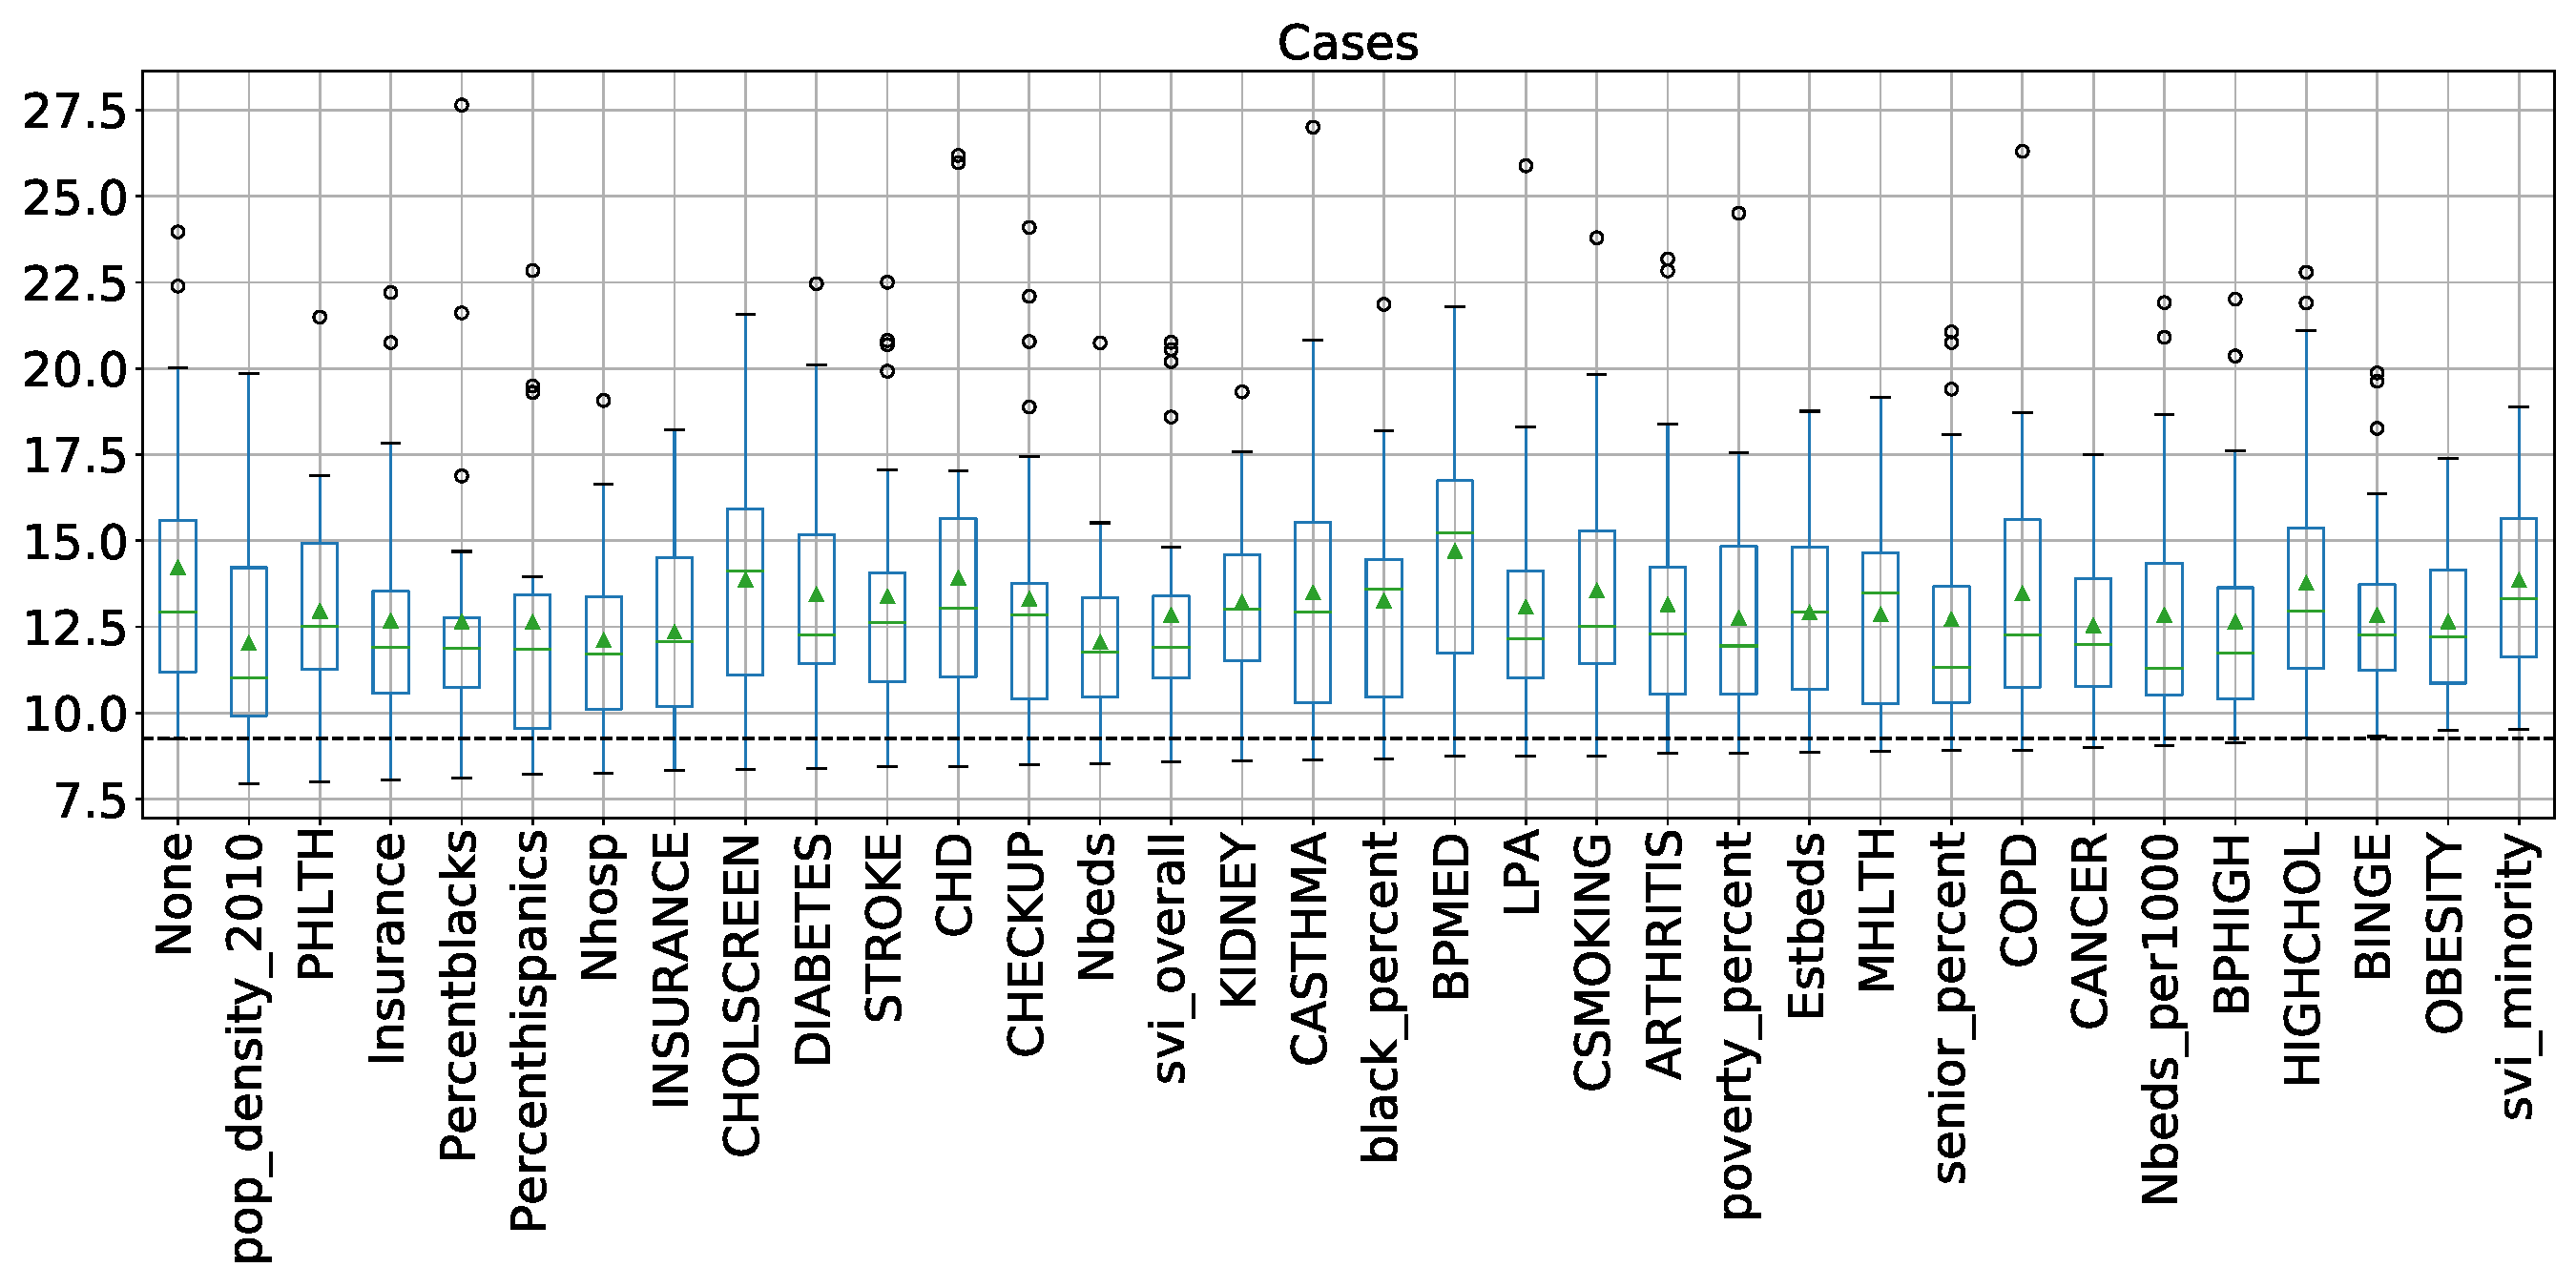
\includegraphics[width=1.0\textwidth]{images/boxwhisker/boxplot_cases.pdf}
    \vspace{-1cm}
    \caption{Influence of risk factors on the accuracy of the prediction of COVID-19 cases. The y-axis represents the cumulative error over all input data for the cities.}
    \label{fig:box-cases}
    \bigskip

    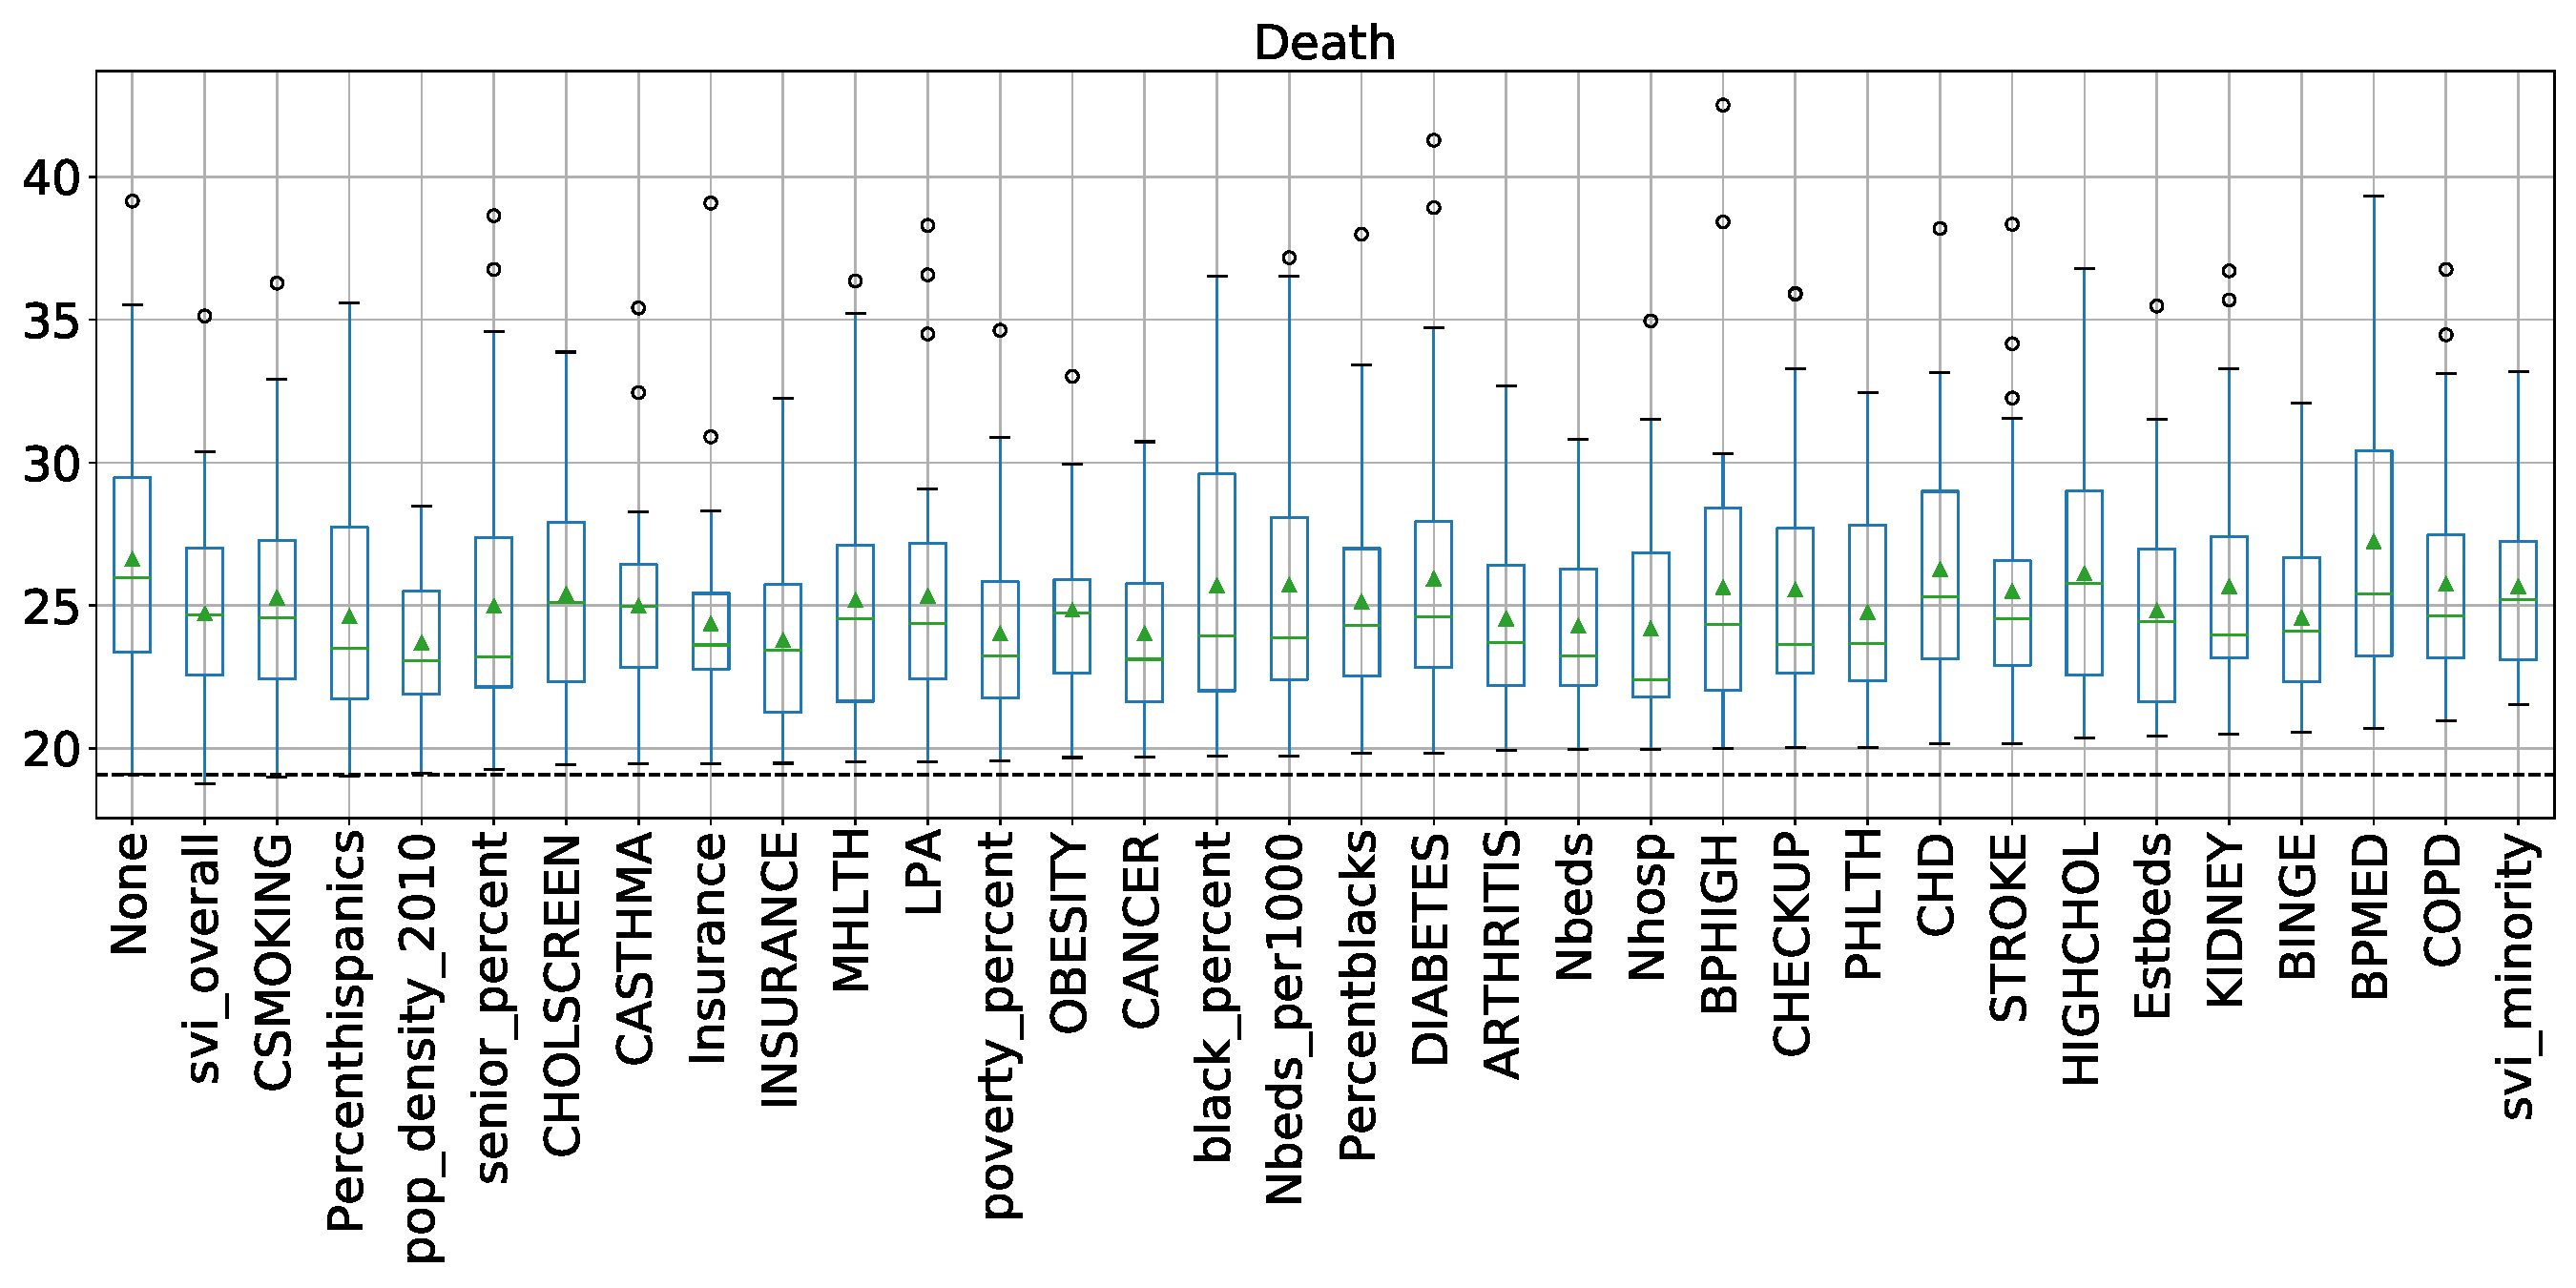
\includegraphics[width=1.0\textwidth]{images/boxwhisker/boxplot_death.pdf}
    \vspace{-1cm}
    \caption{Influence of risk factors on the accuracy of the prediction of COVID-19 death. The y-axis represents the cumulative error over all input data for the cities.}
    \label{fig:box-death}
\end{figure}

%%%%%%


Further, the obtained sorted order of the best prediction models by minimum error based on the risk factors for cases and deaths are as follows:

\begin{description}

\item[Order for cases sorted by minimum model error:] NONE, POP\_DENSITY\_2010, PHLTH, INSURANCE, PERCENTBLACKS, PERCENTHISPANICS, NHOSP, INSURANCE, CHOLSCREEN, DIABETES, STROKE, CHD, CHECKUP, NBEDS, SVI\_OVERALL, KIDNEY, CASTHMA, 
BLACK, BPMED, LPA, CSMOKING, ARTHRITIS, POVERTY, ESTBEDS, MHLTH, SENIOR, COPD, CANCER, NBEDS/1000, BPHIGH, HIGHCHOL, BINGE, OBESITY, SVI\_MINORITY

\item[Order for deaths sorted by minimum model error:]
NONE, SVI\_OVERALL, CSMOKING, PERCENTHISPANICS, POP\_DENSITY\_2010, SENIOR, CHOLSCREEN, CASTHMA, INSURANCE, INSURANCE, MHLTH, LPA, POVERTY, OBESITY, CANCER, BLACK, NBEDS/1000, PERCENTBLACKS, DIABETES, ARTHRITIS, NBEDS, NHOSP, BPHIGH, CHECKUP, PHLTH, CHD, STROKE, HIGHCHOL, ESTBEDS, KIDNEY, BINGE, BPMED, COPD, SVI\_MINORITY
\end{description}

We show the errors and the association with a risk factor in Table \ref{tab:top-1}, where cum\_error represents the cumulative error of the prediction. We sorted it by the cumulative error for cases. We see that in our experiment, almost all risk factors lead to an increased model prediction accuracy. As a result, we note that by including factors such as population density, physical health Insurance, population breakdown by ethnicity, number of hospitals, and diabetes, it leads to better overall predictions for cases. We also see that many of these factors perform better on average.  

\begin{table}[!p]
\caption{Best models for each risk factor and their respective errors. The model that uses no risk factor is highlighted in grey.}
\label{tab:top-1}
\bigskip
\centering
\resizebox{1.0\textwidth}{!}{ 
\begin{tabular}{rrrrrlrl}
\toprule
 \makecell{RMSE\\Cases} &  
 \makecell{RMSE\\Death} &  
 \makecell[r]{Cummulative \\Error \\Cases} &  
 \makecell[r]{Cummulative \\Error \\Death} &  
 \makecell[r]{Number of \\Days as \\Input} & 
 \makecell{Risk Factor} &  
 \makecell{Place/\\Rank} & \\
\midrule
 0.055443 & 0.067617 & 7.94 & 22.74 & 5 & POP\_DENSITY\_2010 & 0 \\
 0.054795 & 0.068529 & 8.01 & 20.55 & 3 & PHLTH & 1 \\
 0.055199 & 0.067641 & 8.07 & 20.43 & 4 & INSURANCE & 2 \\
 0.055028 & 0.067207 & 8.12 & 20.17 & 4 & PERCENTBLACKS & 3 \\
 0.056061 & 0.067489 & 8.22 & 19.04 & 5 & PERCENTHISPANICS & 4 \\
 0.054621 & 0.068255 & 8.26 & 20.10 & 3 & NHOSP & 5 \\
 0.054557 & 0.068572 & 8.34 & 24.61 & 3 & INSURANCE & 6 \\
 0.054712 & 0.069121 & 8.37 & 21.70 & 3 & CHOLSCREEN & 7 \\
 0.054586 & 0.067636 & 8.40 & 20.50 & 5 & DIABETES & 8 \\
 0.054160 & 0.066906 & 8.45 & 20.16 & 4 & STROKE & 9 \\
 0.054027 & 0.067642 & 8.46 & 21.93 & 5 & CHD & 10 \\
 0.054927 & 0.067652 & 8.51 & 20.42 & 5 & CHECKUP & 11 \\
 0.054146 & 0.067536 & 8.54 & 21.15 & 5 & NBEDS & 12 \\
 0.054795 & 0.067676 & 8.58 & 19.94 & 5 & SVI\_OVERALL & 13 \\
 0.054600 & 0.067565 & 8.61 & 21.86 & 5 & KIDNEY & 14 \\
 0.055089 & 0.068248 & 8.63 & 22.58 & 5 & CASTHMA & 15 \\
 0.054547 & 0.068266 & 8.68 & 20.49 & 3 & BLACK & 16 \\
 0.054685 & 0.068920 & 8.74 & 21.69 & 3 & BPMED & 17 \\
 0.054323 & 0.067149 & 8.75 & 19.54 & 5 & LPA & 18 \\
 0.053716 & 0.066898 & 8.75 & 19.01 & 5 & CSMOKING & 19 \\
 0.054053 & 0.068716 & 8.83 & 20.94 & 3 & ARTHRITIS & 20 \\
 0.055029 & 0.068672 & 8.84 & 22.02 & 3 & POVERTY & 21 \\
 0.054545 & 0.067267 & 8.86 & 21.22 & 4 & ESTBEDS & 22 \\
 0.054864 & 0.068742 & 8.90 & 19.53 & 3 & MHLTH & 23 \\
 0.055079 & 0.069024 & 8.93 & 21.23 & 3 & SENIOR & 24 \\
 0.055589 & 0.068250 & 8.93 & 23.26 & 4 & COPD & 25 \\
 0.054500 & 0.068363 & 8.99 & 19.70 & 3 & CANCER & 26 \\
 0.054397 & 0.068491 & 9.05 & 21.89 & 3 & NBEDS/1000 & 27 \\
 0.054609 & 0.067346 & 9.13 & 21.29 & 4 & BPHIGH & 28 \\
\rowcolor{black!5}  0.054868 & 0.069432 & 9.26 & 25.88 & 3 & NONE & 29 \\
 0.056429 & 0.069345 & 9.28 & 20.98 & 3 & HIGHCHOL & 30 \\
 0.054317 & 0.067638 & 9.32 & 21.00 & 5 & BINGE & 31 \\
 0.054469 & 0.068540 & 9.50 & 20.65 & 3 & OBESITY & 32 \\
 0.055094 & 0.067443 & 9.54 & 21.53 & 4 & SVI\_MINORITY & 33 \\
\bottomrule
\end{tabular}
}
\end{table}

We observed a different scenario for deaths, in which we only identified two risk factors, namely the Social Vulnerability Index (SVI) and chain-smoking, that, when integrated into our deep learning model, leads to better prediction results. However, the accuracy of the overall prediction of deaths is far less precise than that of the cases. To showcase this, we have included Figures \ref{fig:error-case-popdensity} and \ref{fig:error-death-popdensity} that show the respective errors. 

\begin{figure}[!h]
    \begin{minipage}{.45\textwidth}
    \centering
    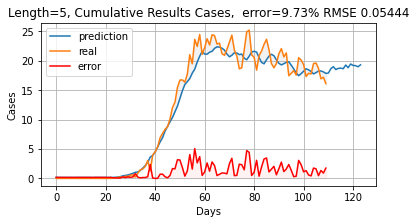
\includegraphics[width=1.0\textwidth]{images/predict/Length_5-fields_pop_density_2010-Cumulative-Cases.png}
    \vspace{-1cm}
    \caption{Model prediction error for cumulative cases when including one risk factor - POP\_DENSITY\_2010 in the features, in addition to the past number of cases and deaths.}
    \label{fig:error-case-popdensity}
    \end{minipage}
    \begin{minipage}{.45\textwidth}
    \ \
    \centering
    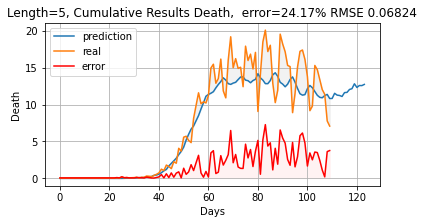
\includegraphics[width=1.0\textwidth]{images/predict/Length_5-fields_pop_density_2010-Cumulative-Death.png}
    \vspace{-1cm}
    \caption{Model prediction error for cumulative deaths when including one risk factor - POP\_DENSITY\_2010  in the features, in addition to the past number of cases and deaths.}
    \label{fig:error-death-popdensity}
    \end{minipage}
\end{figure}


This is following our input data distribution in which we noted higher fluctuations relative to the overall value. A mitigation to this issue would be using a seven day average over the analyzed period. However, we have not done this on purpose for this analysis as we wanted to identify how a covariate enhanced LSTM behaves that includes risk factors based on the daily fluctuations. This was done to avoid and showcase any needed preproccessing on the data and to identify the capability of the deep learning framework while adapting to the fluctuations without any special activities. Previously, we have already shown in Section \ref{sec:emperical} that for smooth data inputs the prediction is very accurate.
Using fluctuation data allows our framework for an automated ingest of data on a daily basis to enable data fusion of new cases and death information. Hence, we can re-train the model with new incoming data every day. Through repeated training experiments, we found the LSTM hyperparameters such as epochs and dropout values that work well for our experiments.

We conducted one additional analysis and plotted the best risk factor prediction model errors, the five best, and the ten best from our experiments to identify if we have better predictions than by including no risk factor. The best result found with no risk factor is depicted with the black horizontal line. Figures~\ref{fig:place-top1-cases} to  \ref{fig:place-top10-death} show the results sorted by the minimized error. Notably, we identified that a jump occurs when we sort the top 10 model predictions at around 330 models from a total of 3400 automatically generated models. This also underscores the need to run our deep learning model multiple times to obtain best parameter candidates. 




\begin{figure}[!h]
    \begin{minipage}{.45\textwidth}
        \centering
        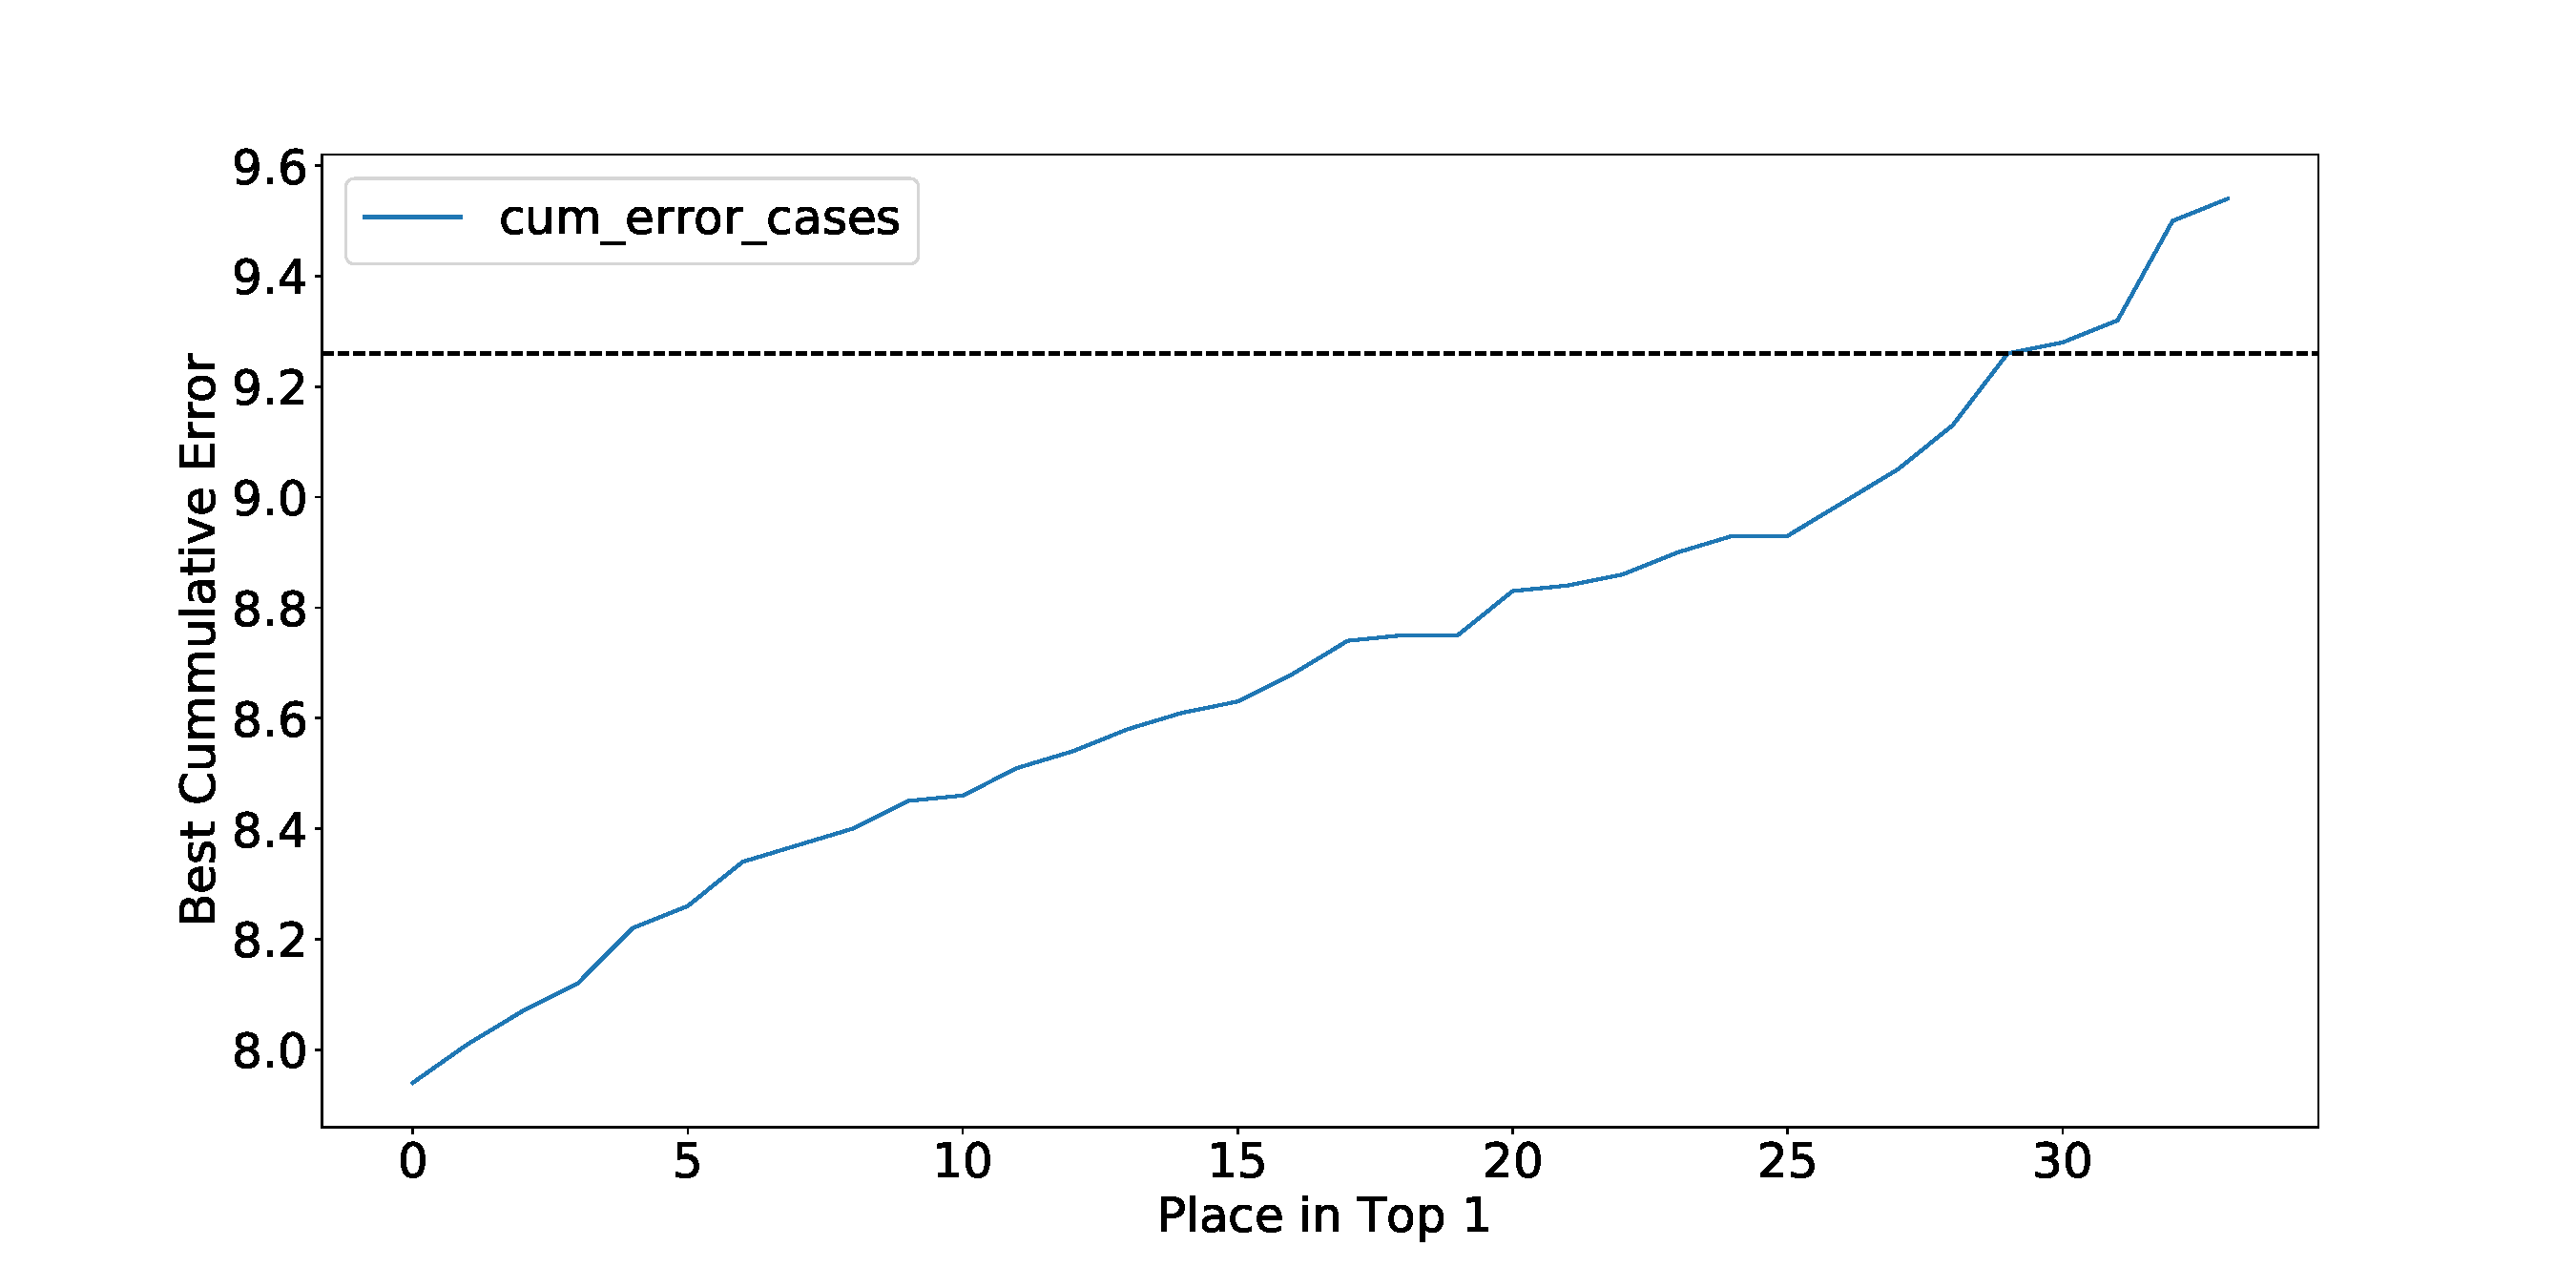
\includegraphics[width=1.0\textwidth]{images/predict/PlaceTop1_Cases.pdf}
        \vspace{-1cm}
        \caption{Best predictions for cases over all risk factors.}
        \label{fig:place-top1-cases}

    \end{minipage}
    \ \
    \begin{minipage}{0.45\textwidth}
        \centering
        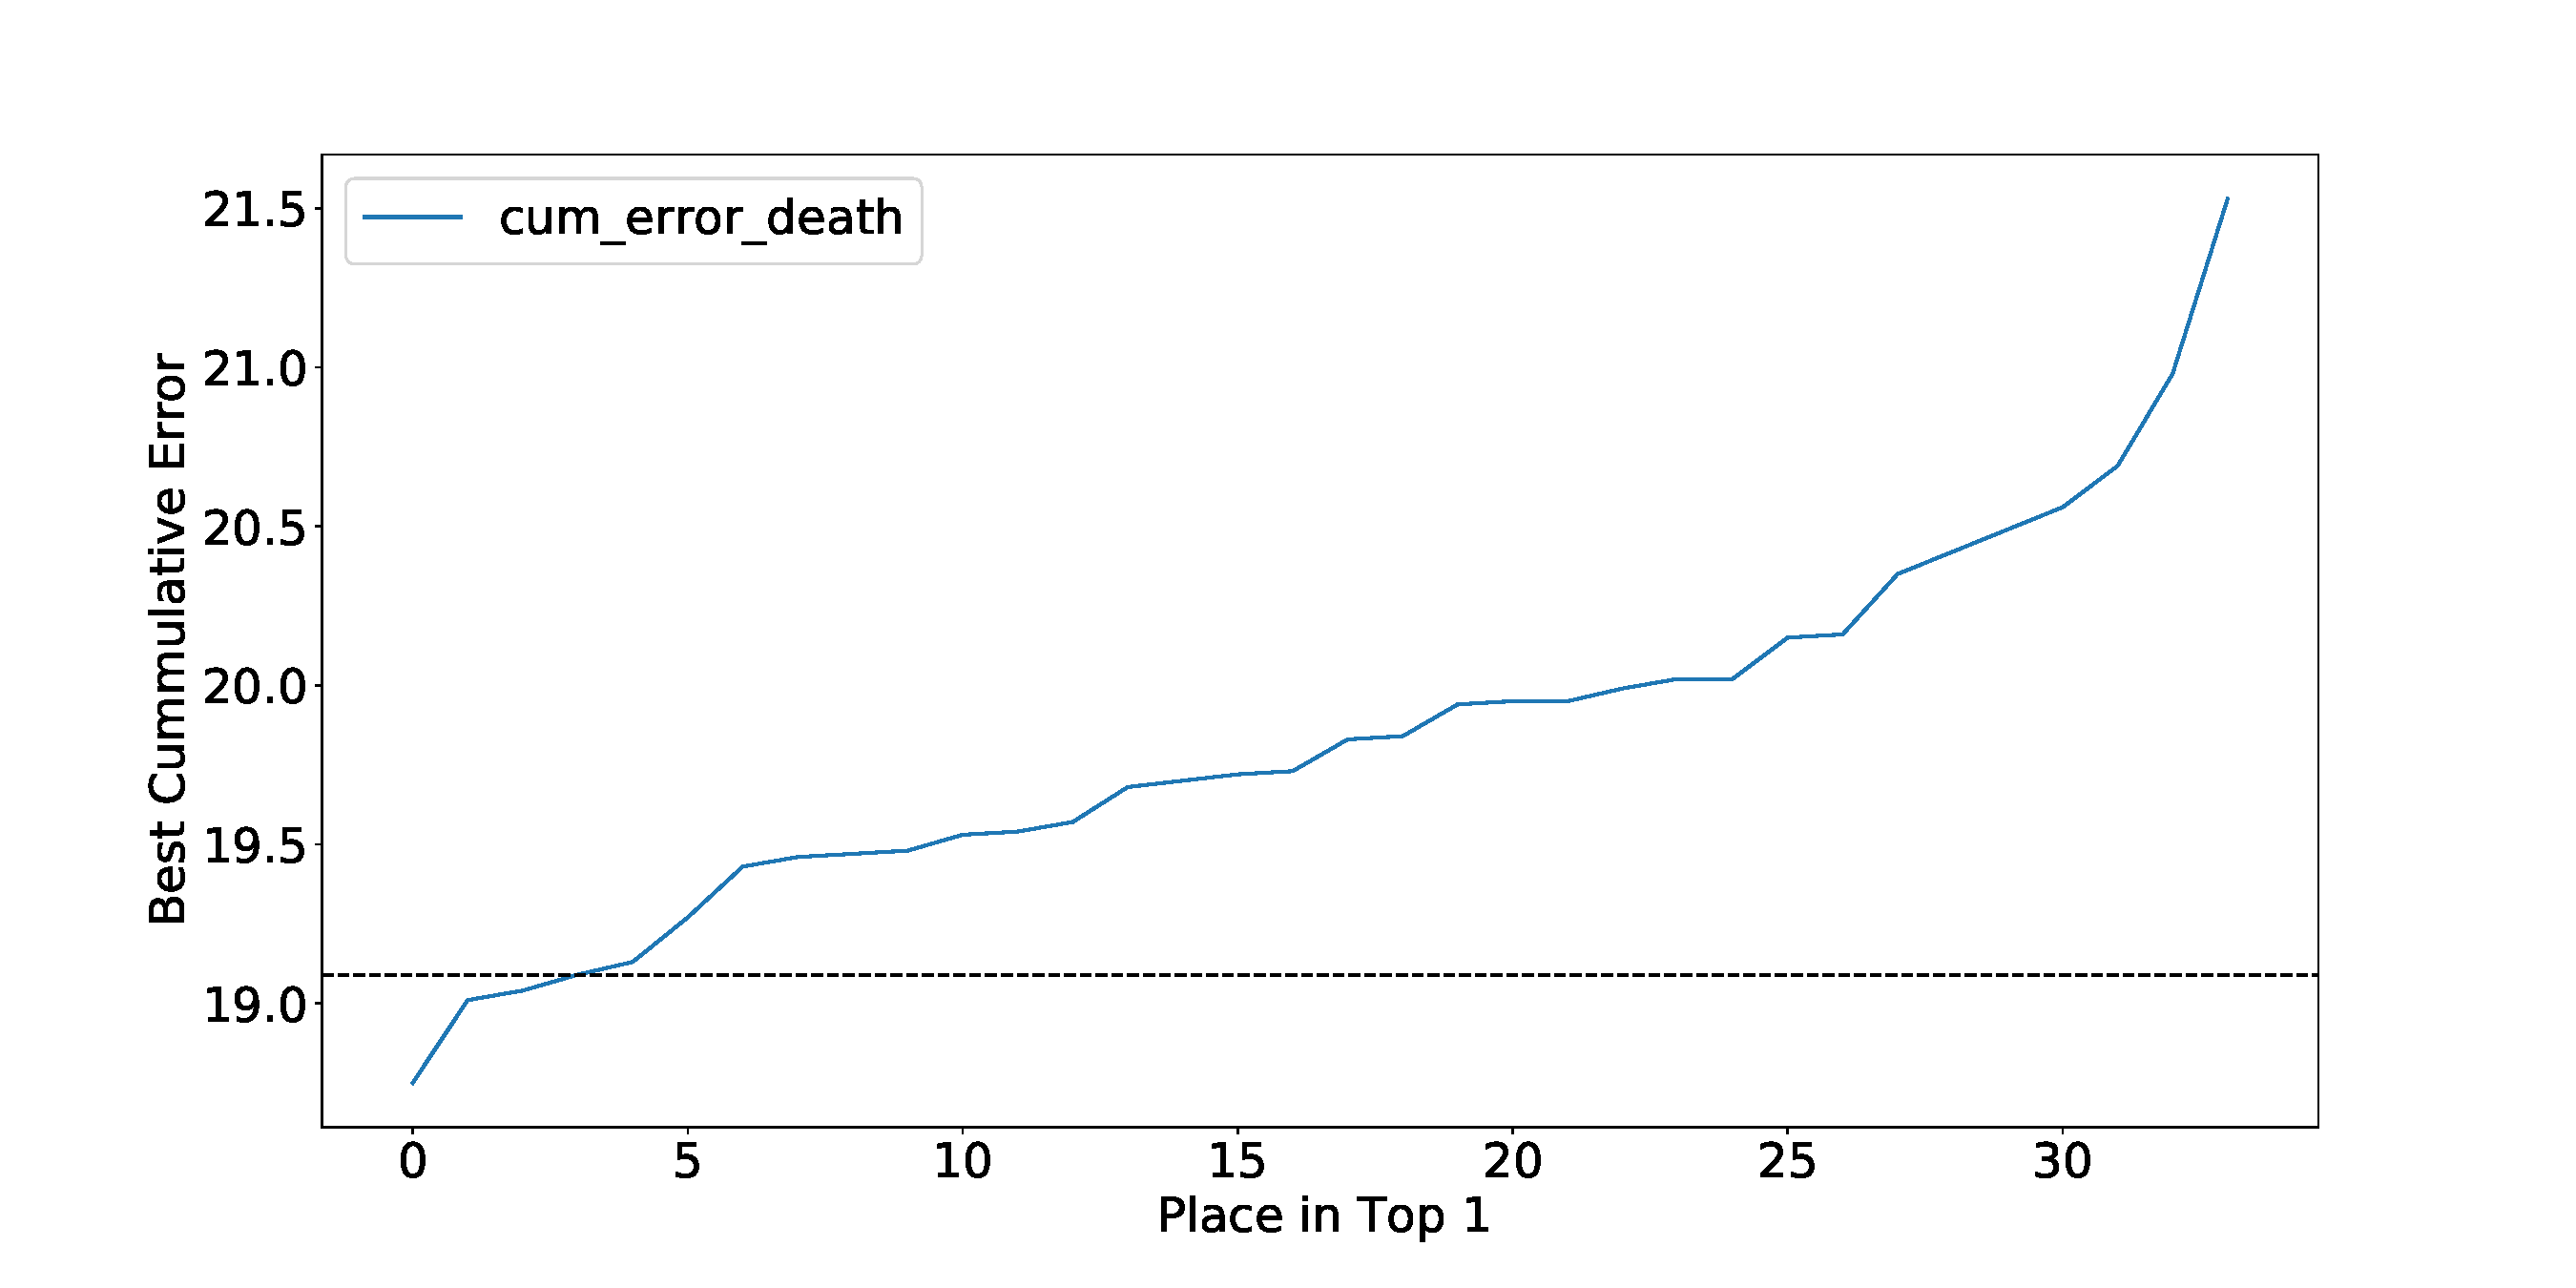
\includegraphics[width=1.0\textwidth]{images/predict/PlaceTop1_Death.pdf}
        \vspace{-1cm}
        \caption{Best predictions for deaths over all risk factors.}
        \label{fig:place-top1-death}
    \end{minipage}

    \begin{minipage}{.45\textwidth}
        \centering
        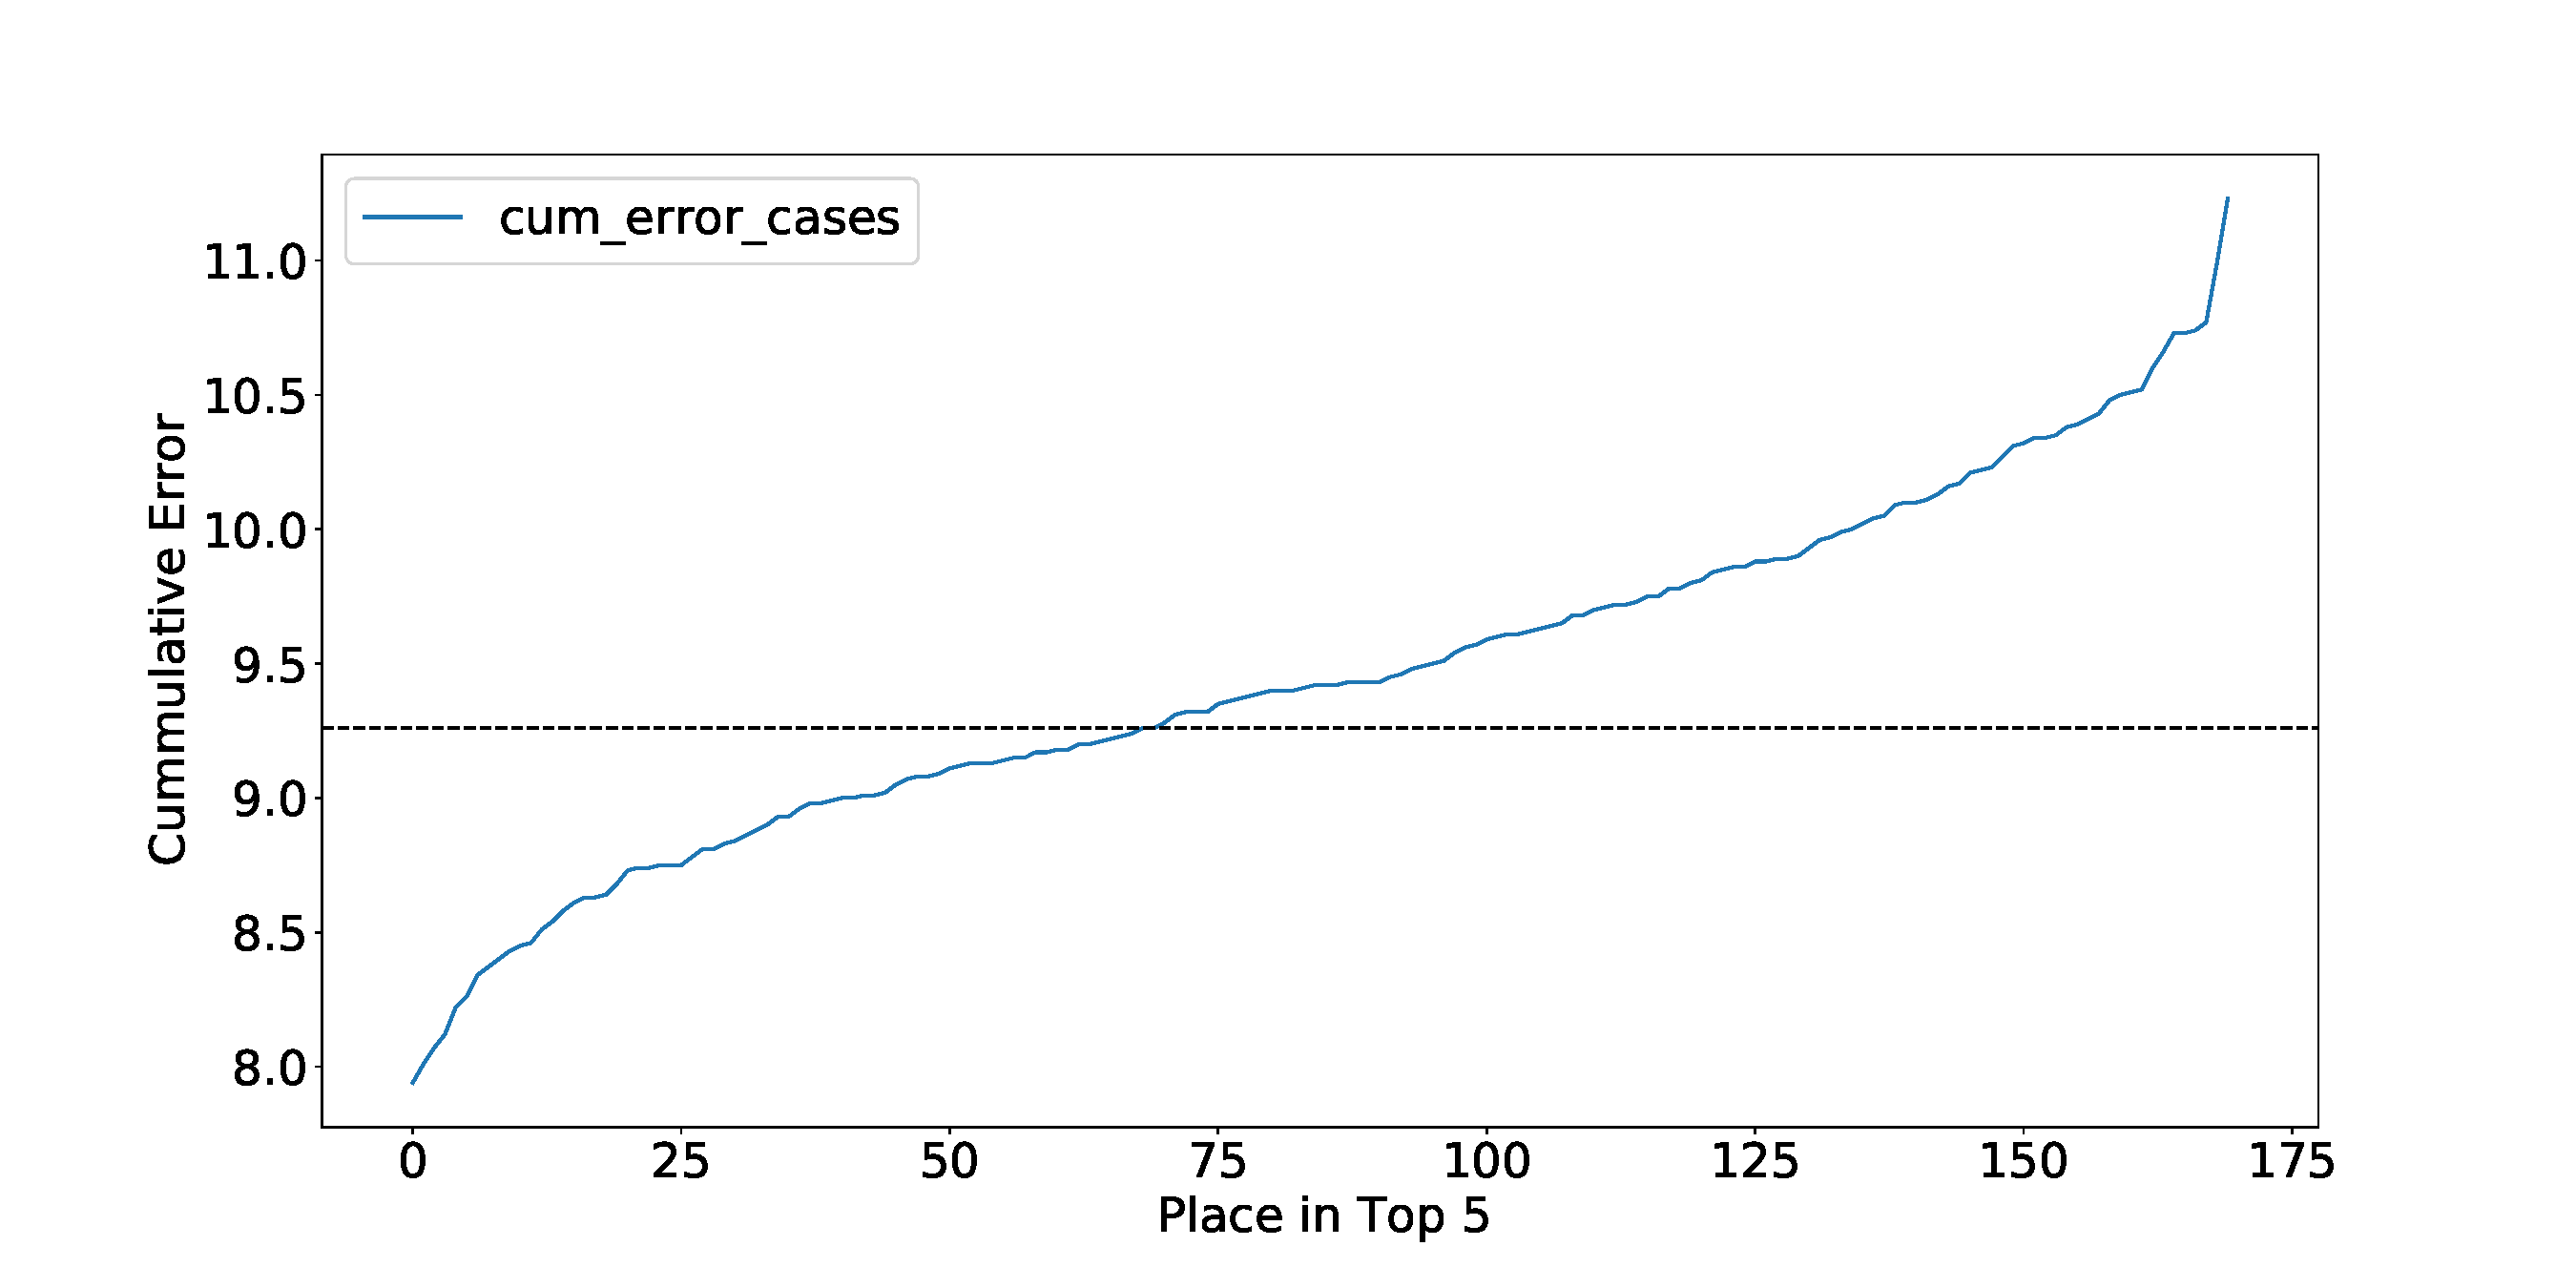
\includegraphics[width=1.0\textwidth]{images/predict/PlaceTop5_Cases.pdf}
        \vspace{-1cm}
        \caption{Top 5 predictions from all cases over all risk factors.}
        \label{fig:place-top5-cases}
    \end{minipage}
    \ \
    \begin{minipage}{.45\textwidth}
        \centering
        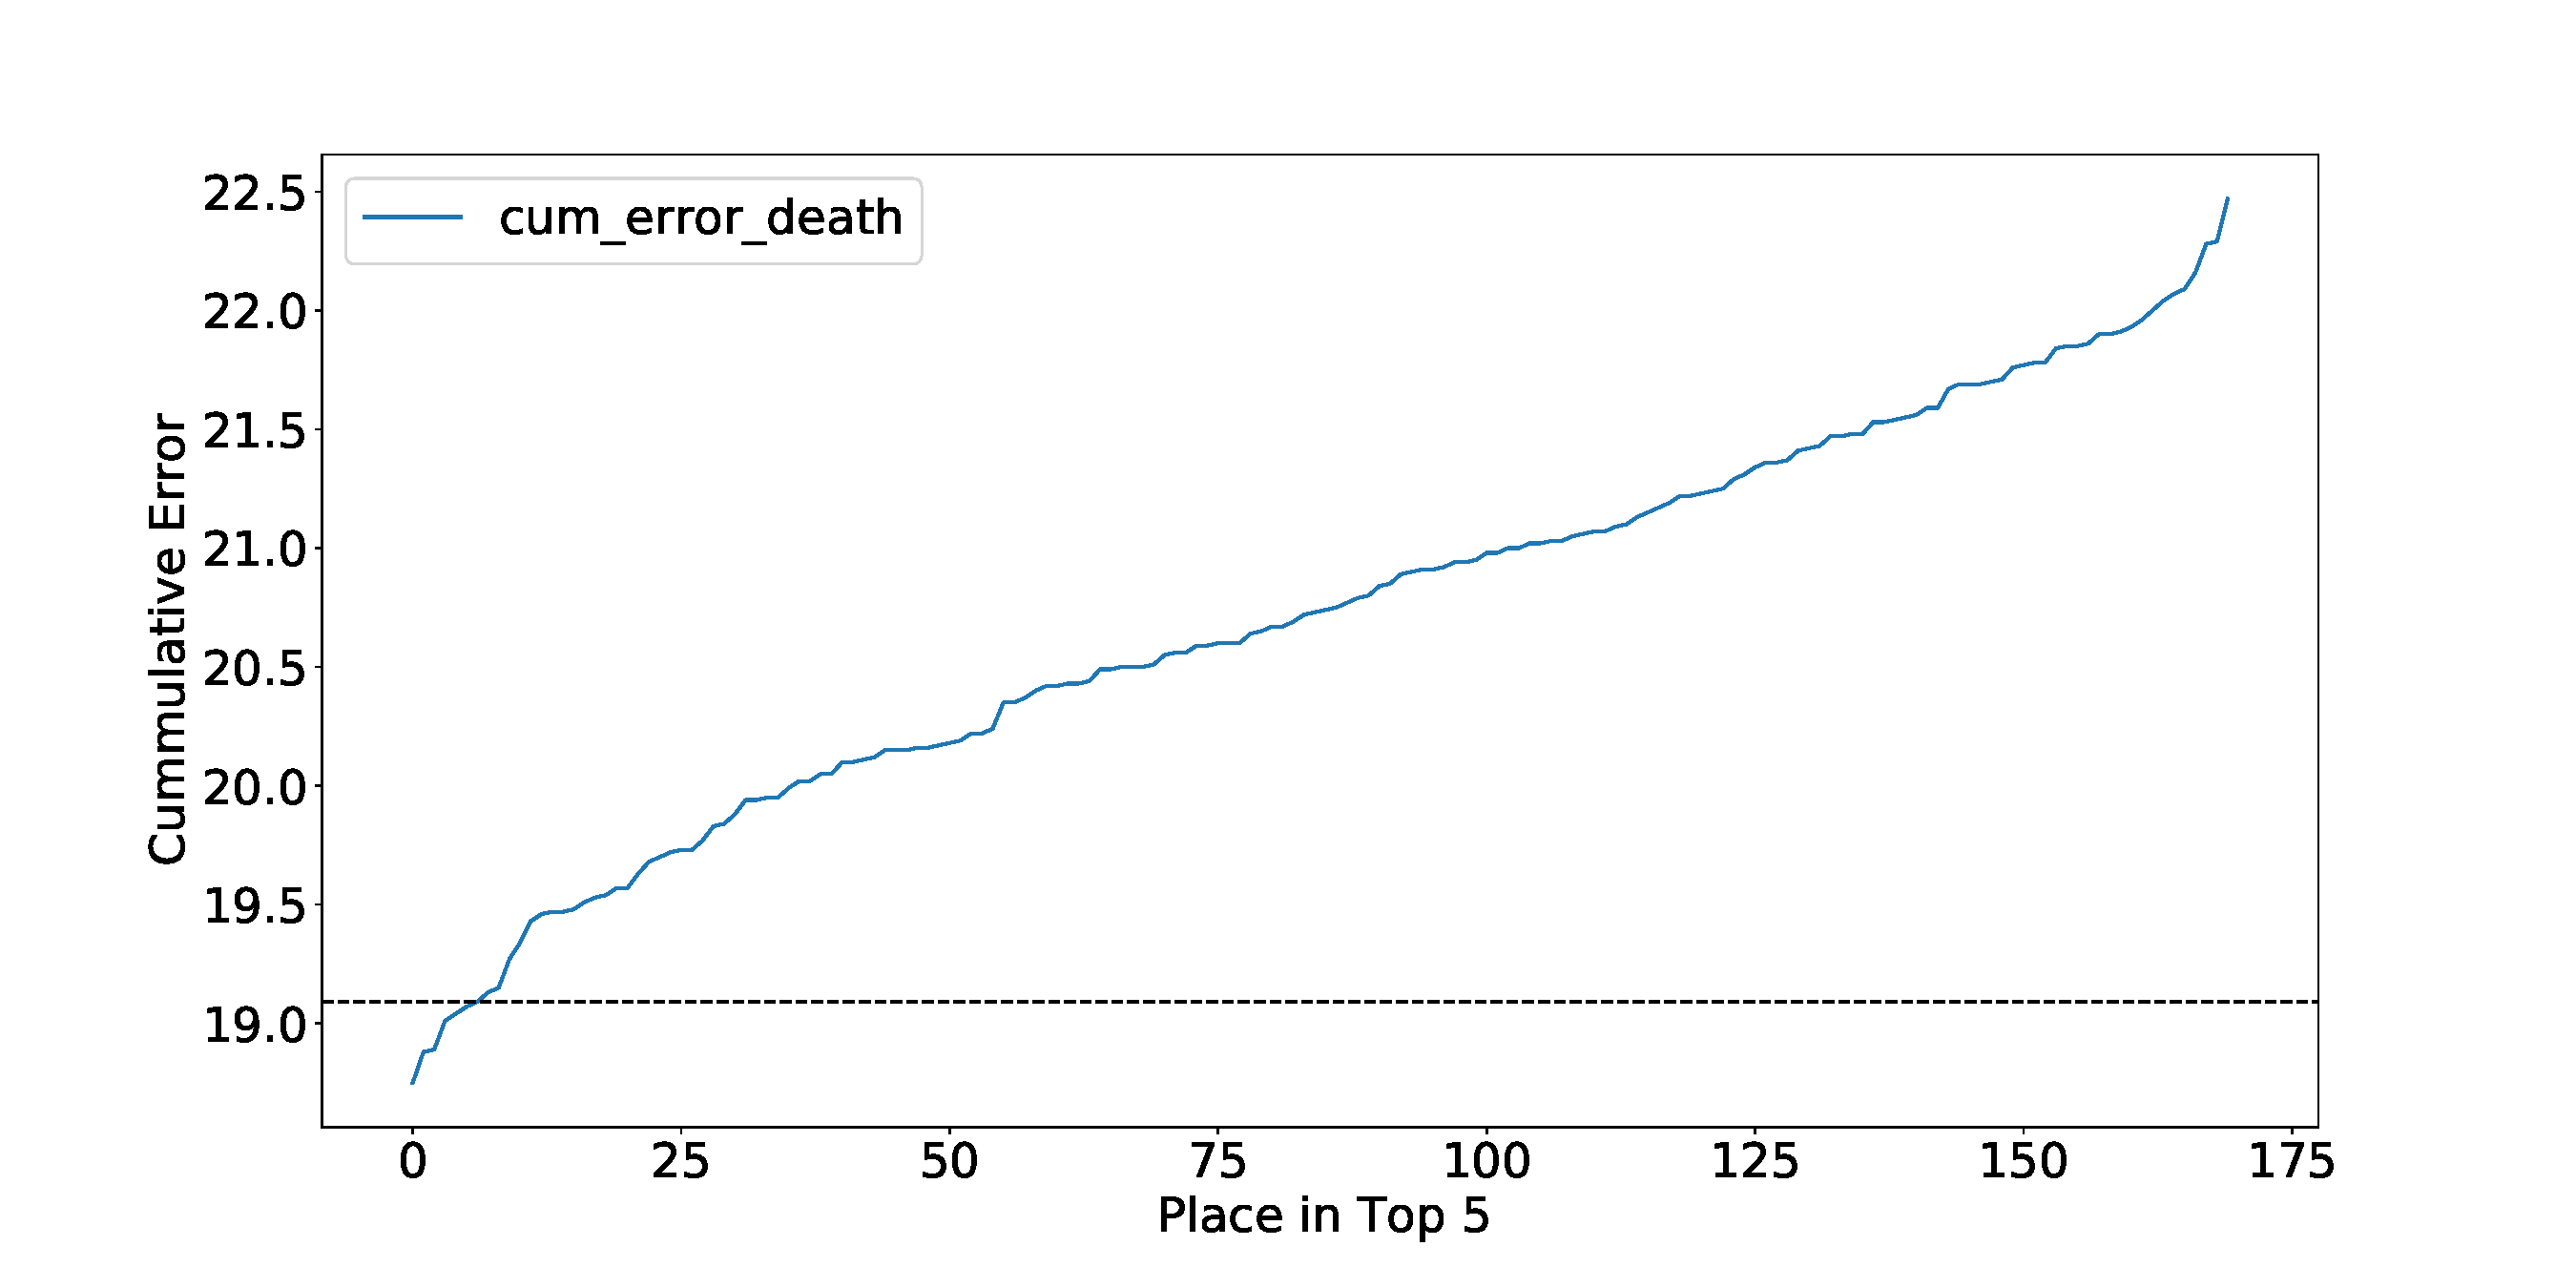
\includegraphics[width=1.0\textwidth]{images/predict/PlaceTop5_Death.pdf}
        \vspace{-1cm}
        \caption{Top 5 predictions from all deaths  over all risk factors.}
        \label{fig:place-top5-death}
    \end{minipage}

    \begin{minipage}{.45\textwidth}
        
        \centering
        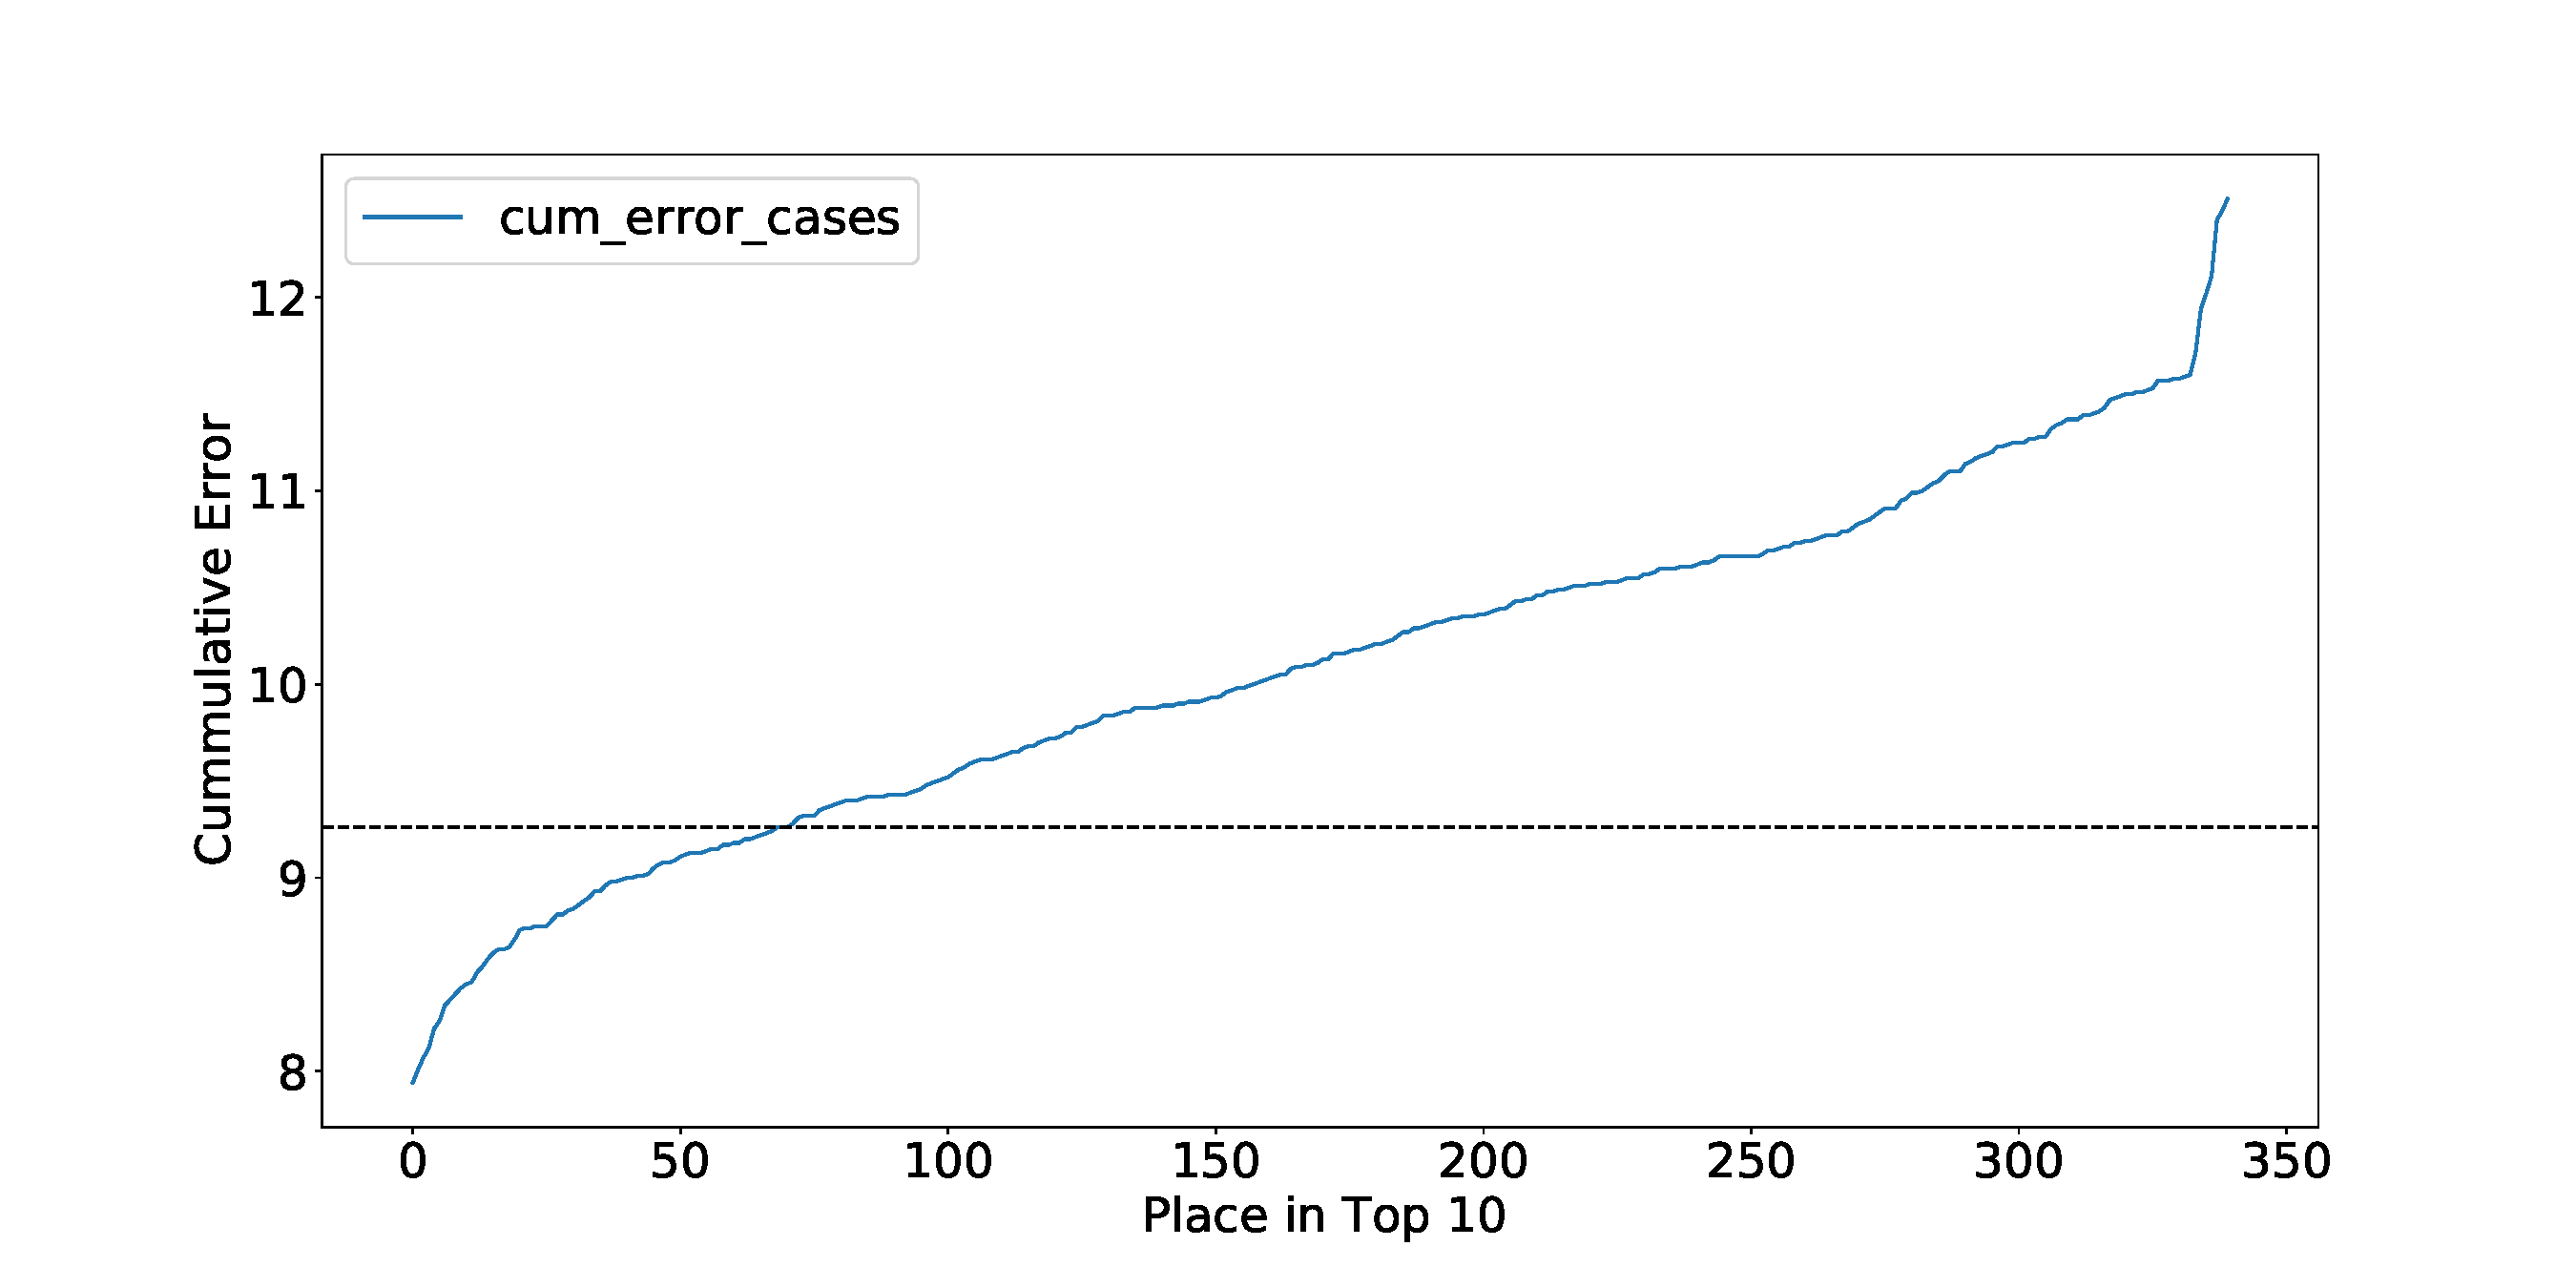
\includegraphics[width=1.0\textwidth]{images/predict/PlaceTop10_Cases.pdf}
        \vspace{-1cm}
        \caption{Top 10 predictions from all deaths  over all risk factors.}
        \label{fig:place-top10-cases}
    \end{minipage}
    \ \
    \begin{minipage}{.45\textwidth}
        
        \centering
        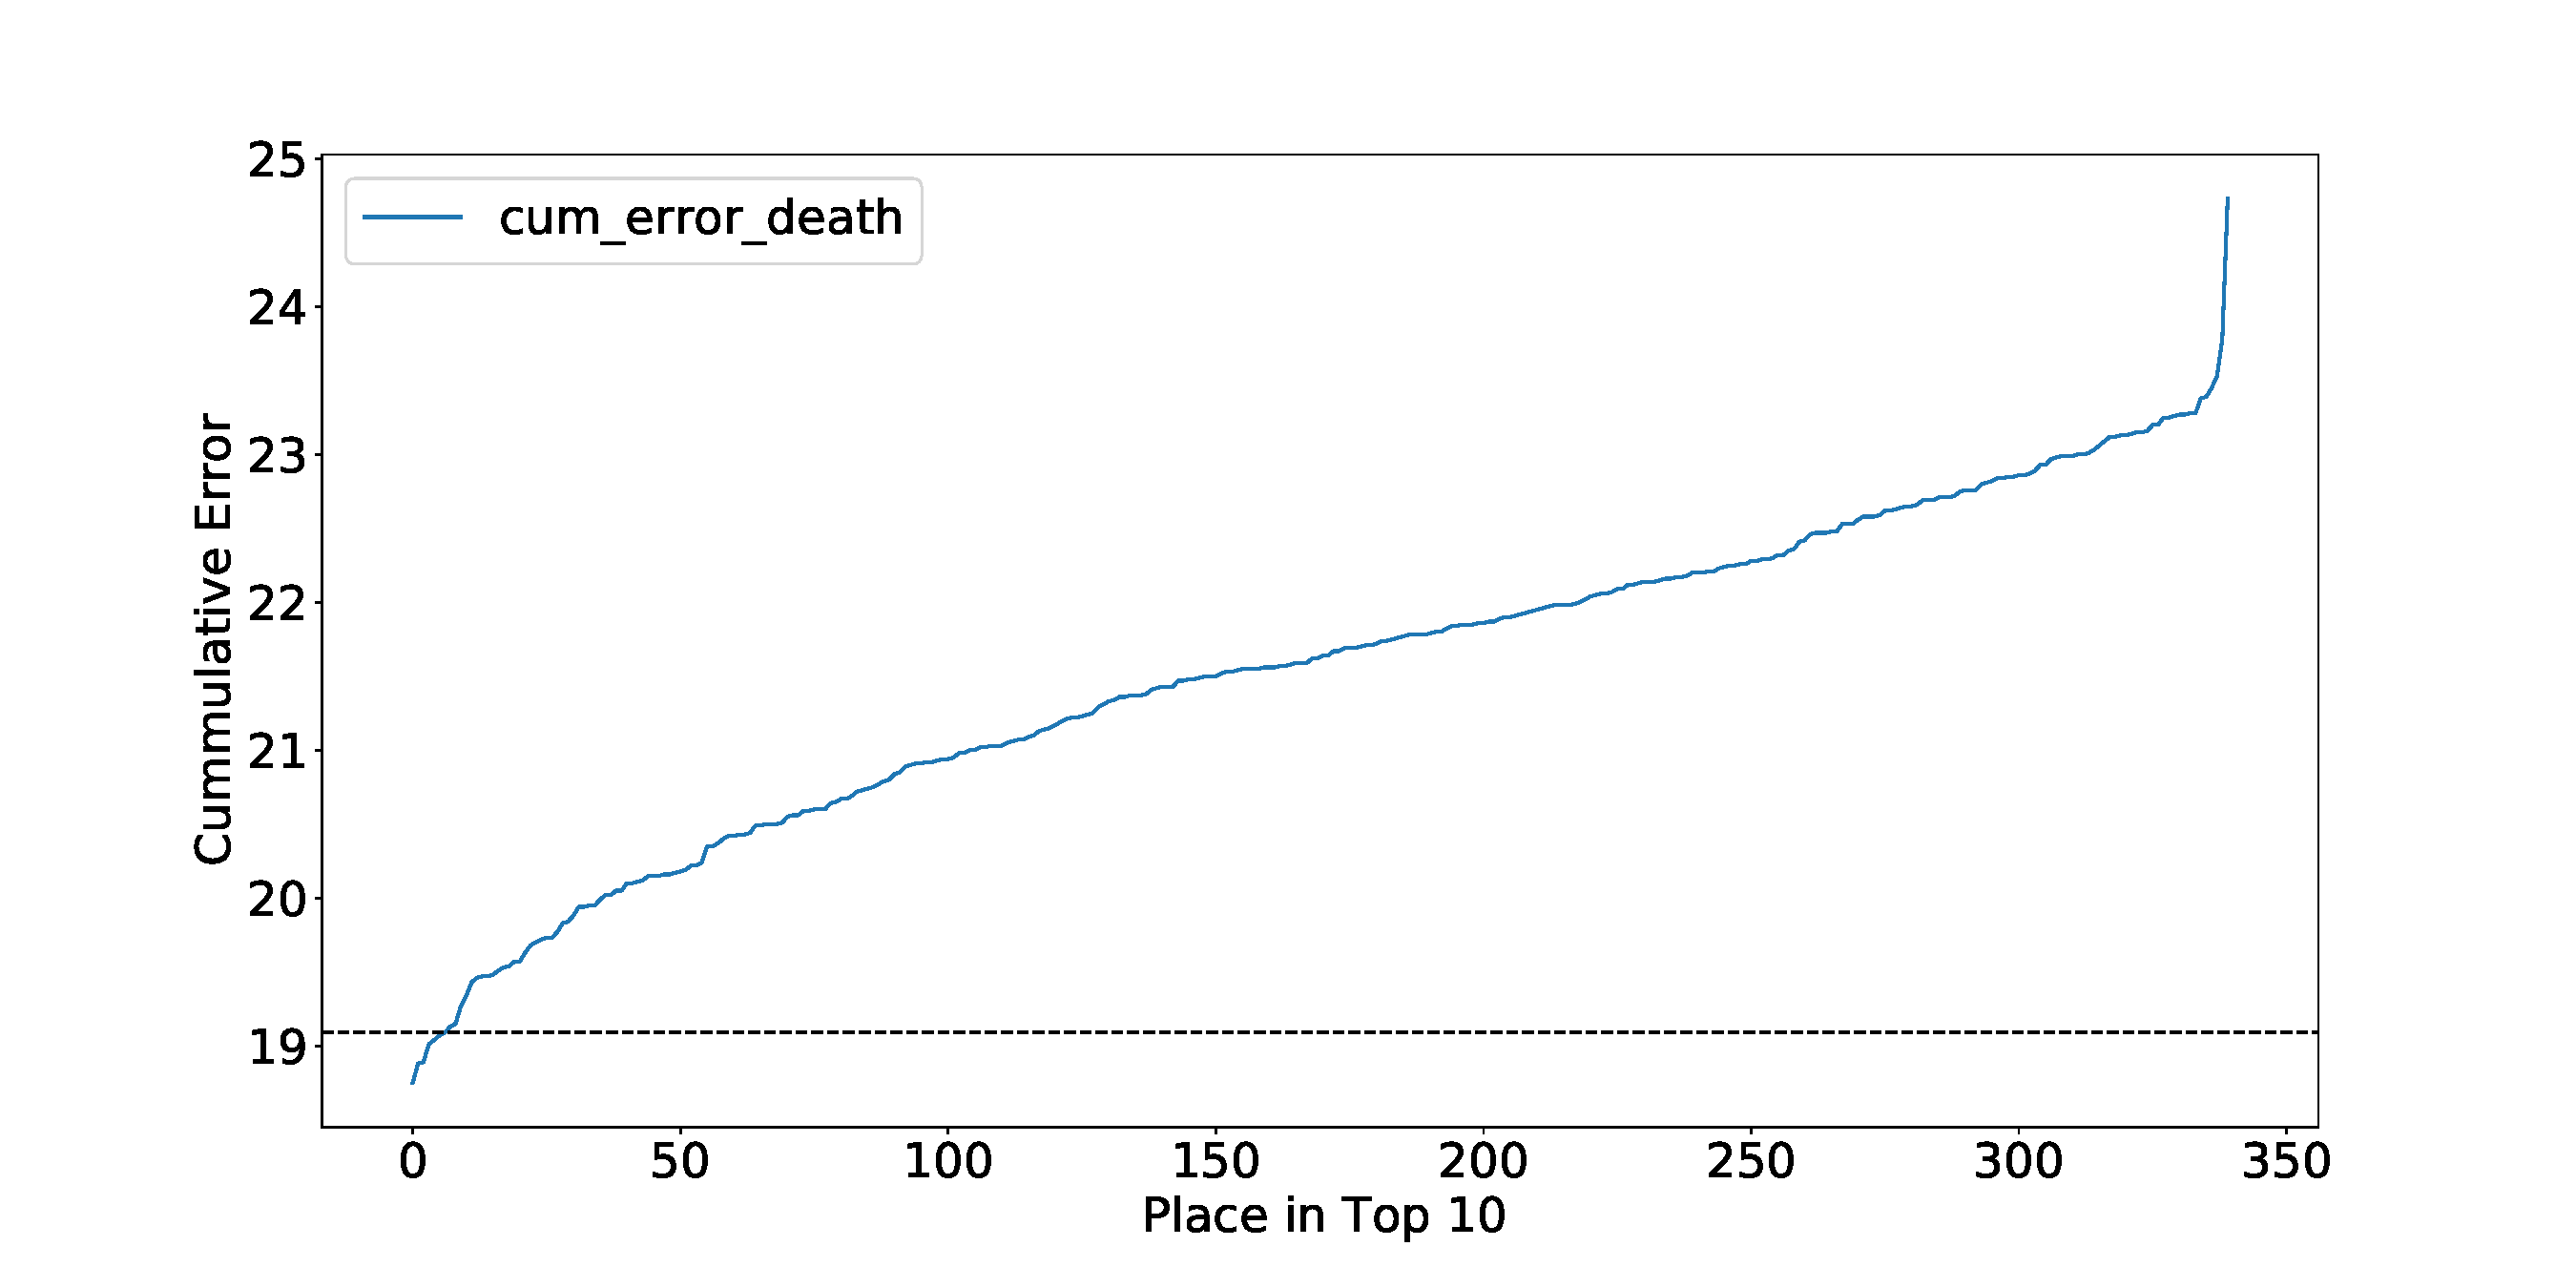
\includegraphics[width=1.0\textwidth]{images/predict/PlaceTop10_Death.pdf}
        \vspace{-1cm}
        \caption{Top 10 predictions from all deaths over all risk factors.}
        \label{fig:place-top10-death}
    \end{minipage}
\end{figure}

\begin{comment}
\begin{figure}[!h]
    \centering
    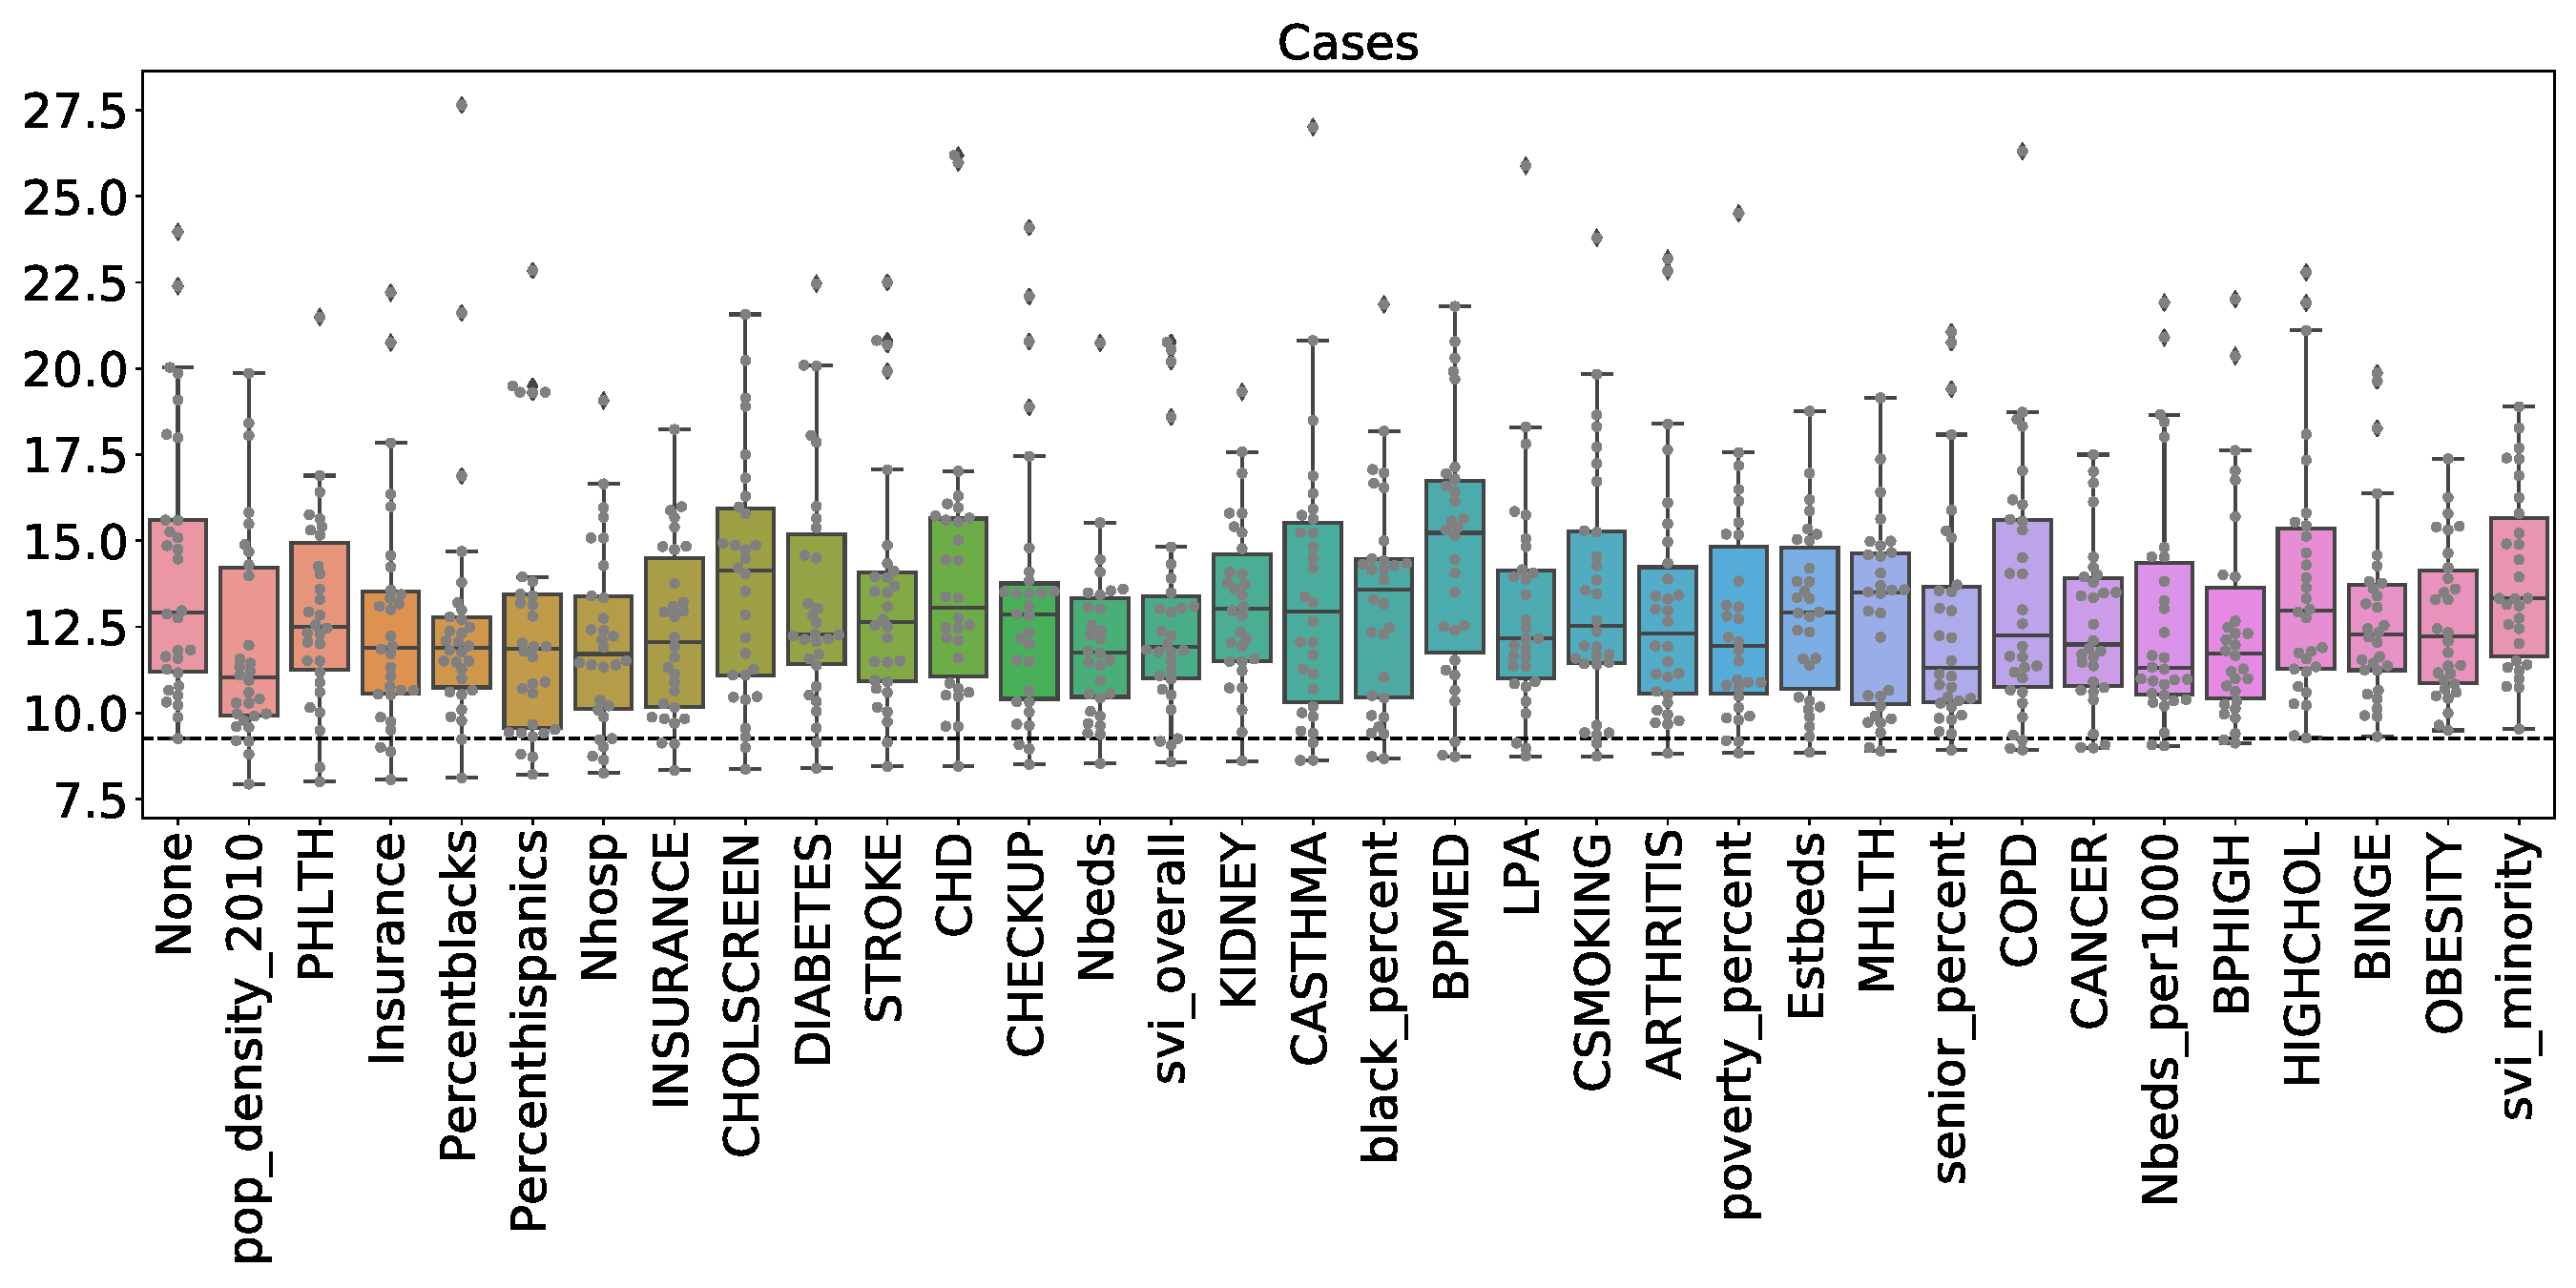
\includegraphics[width=1.0\textwidth]{images/boxwhisker/swarmplot_cases.pdf}
    \caption{Caption}
    \label{fig:my_label}

    \centering
    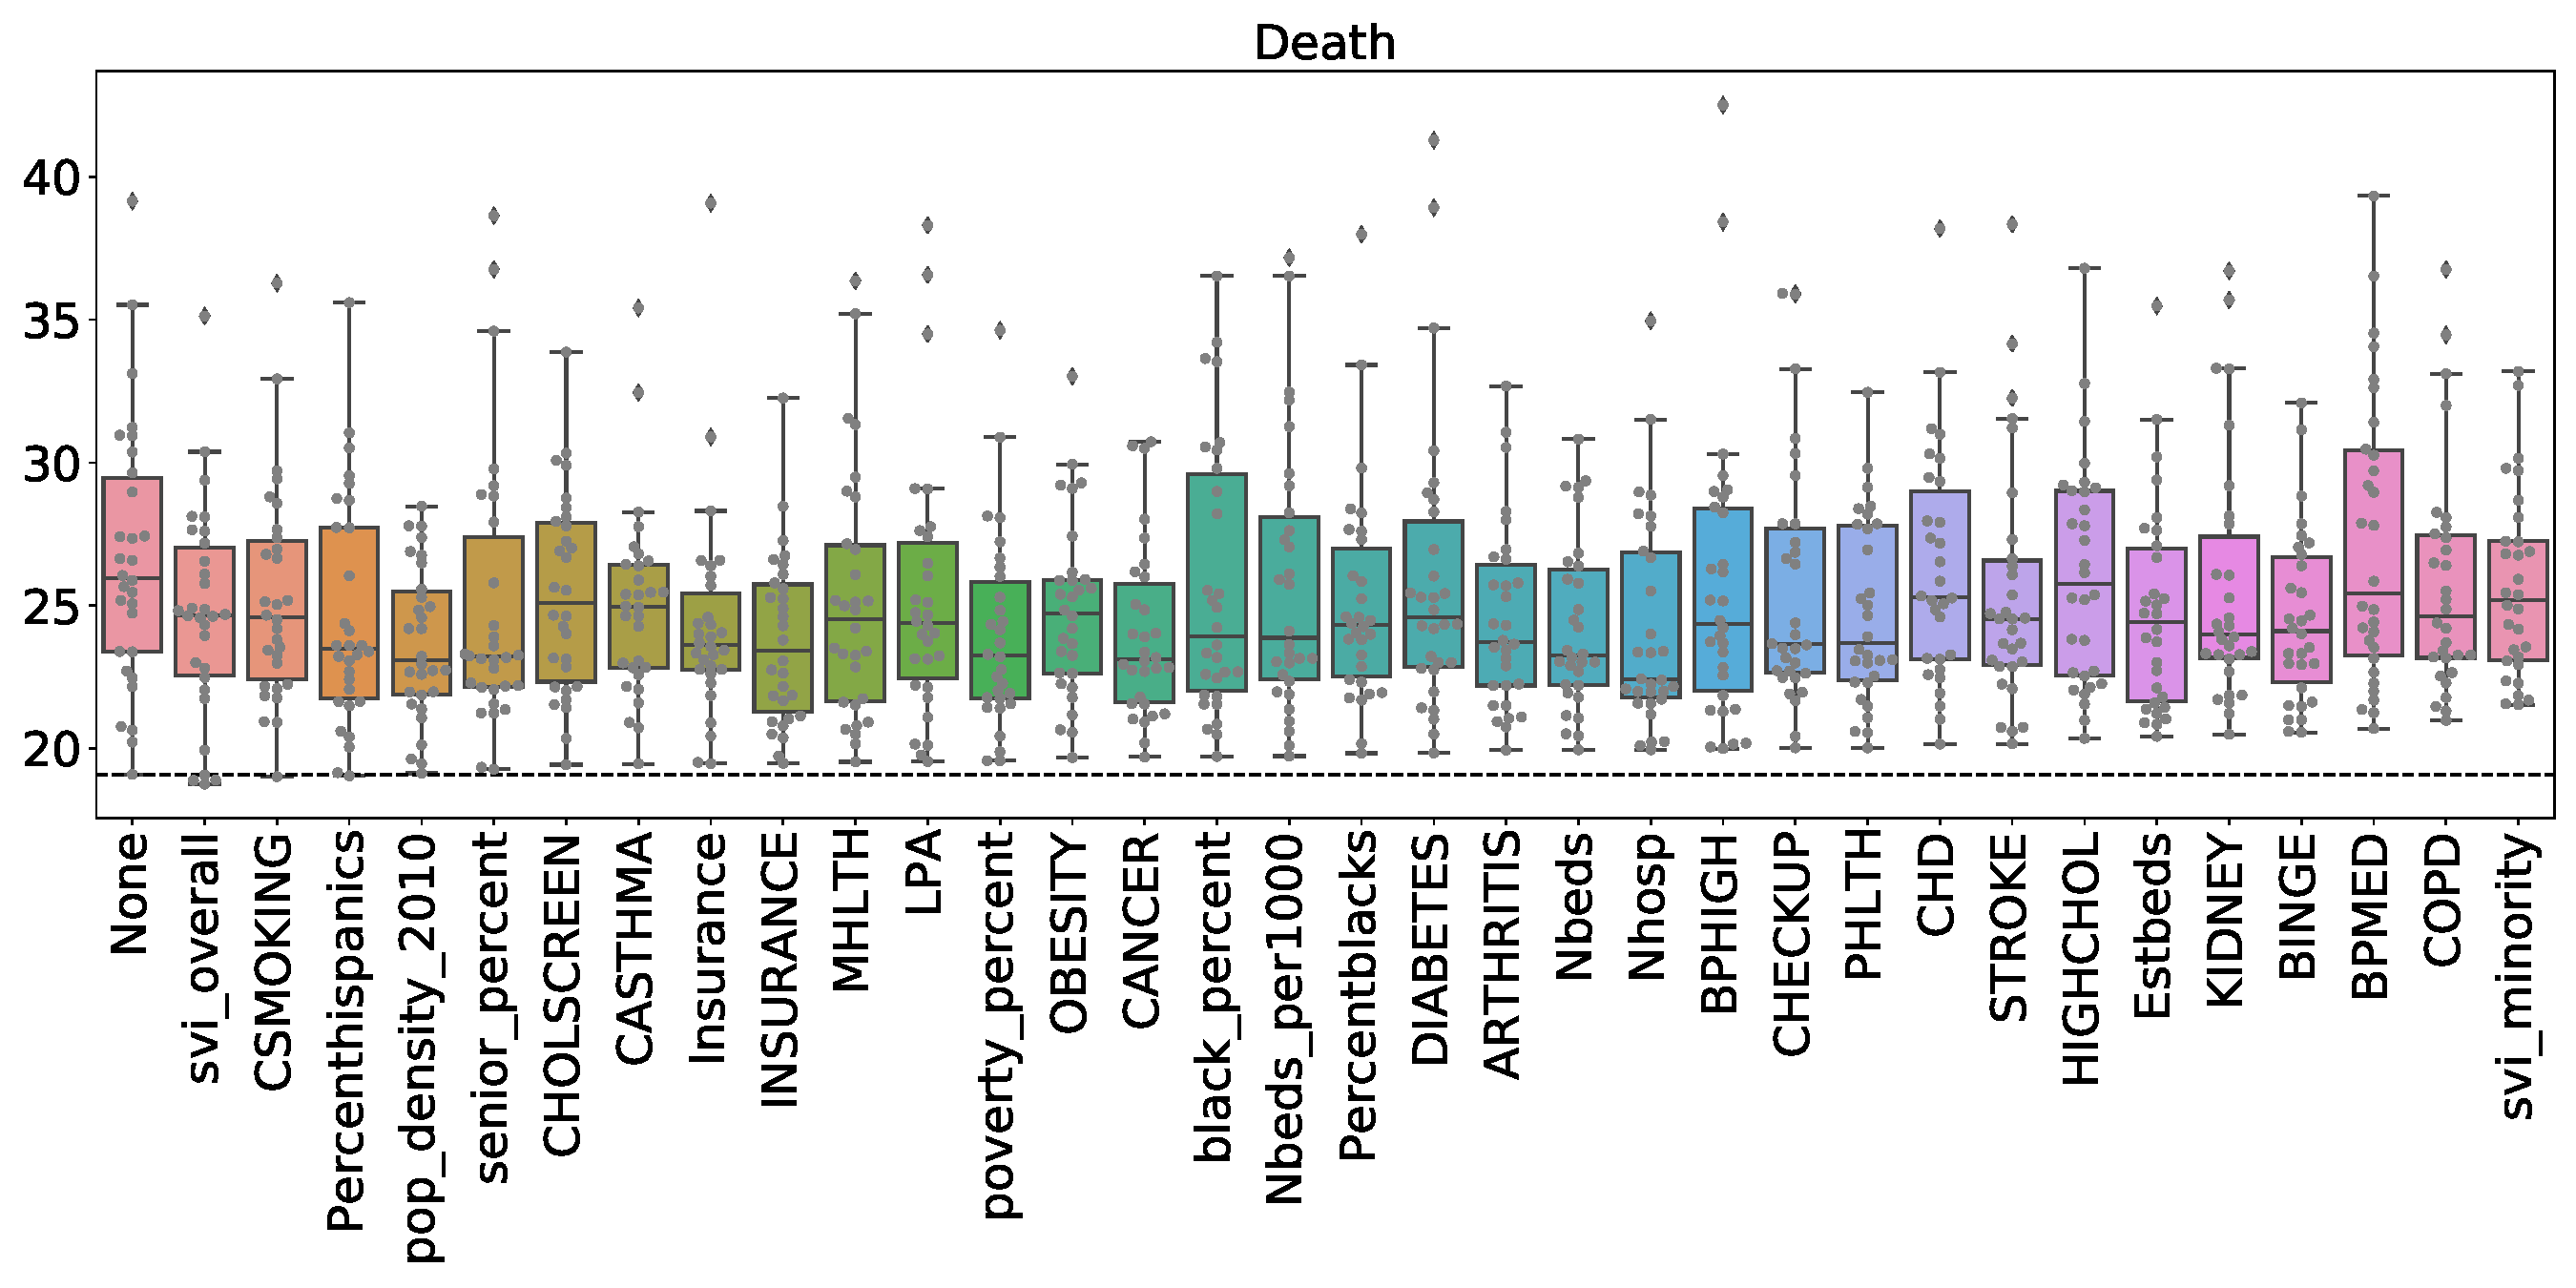
\includegraphics[width=1.0\textwidth]{images/boxwhisker/swarmplot_death.pdf}
    \caption{Caption}
    \label{fig:my_label}
\end{figure}
\end{comment}


While this study focuses on if and which risk factors can improve the predictions, we do not focus on why. Such analysis could provide insights into causal relationships. For example,  information such as health insurance and the number of hospitals and beds are often related to the quality of services that affect early detection and treatment. Furthermore, population parameters such as density can determine the rate of spread and the number of cases. Similarly, distributions of comorbidities in a given population such as physical health, cholesterol screening, diabetes, etc., are found to be insightful in predicting outcomes \cite{Maleki}. Identifying such risk factors and correlating them to the prediction accuracy provides valuable candidates for future studies.



\subsection{Impact and Design of a Multi-Covariate-LSTM}
\label{sec:lstm-many}

In our next comprehensive analysis, we try to answer Question \ref{q:4} if all risk factors impact the analysis. Thus we feed the covariates into the recurrent network as additional features. In addition to cases and deaths, this leads to 35 variables, including 33 unique covariates. We looked at two related ways of doing this:

\begin{description}

\item [(a)] Have covariates fixed in time (static)

\item[(b)] Multiply the covariates by the times series (we used the average of cases and deaths)

\end{description}

We expected the second choice to be the most natural as it gives all
35 input streams similar time dependence. However, in our initial
tests, we found these choices gave very similar results, and so we
focused on the simpler choice (a) in this paper. In the experiments discussed
here, we either used 0, 1, or 33 covariates. Choosing 33 gives the best
description (reducing loss by about 1\%) while using each covariate as
a solitary extra feature allows us a rather sensitive study of the
importance of each individual covariate as we noted in Section \ref{sec:lstm-covariate}.

The final choice was the quantities to predict and train
on. We choose this to be both the cases and deaths values at the
time value following the sequence combined with the same quantities
for the following 14 days. This gives us 30 different output features
for each sequence. We renormalized, so the two basic features
(following day) contributed 50\% of the loss function. We supported
this in TensorFlow with a custom mean square error ($MSE$) loss
function that dropped training values that were not available for time
sequences near the end of the examined period. While one can not
train on future values, we can predict them, as seen in our sample
outputs. We extensively studied both 2 and 30 output features, and they
give similar descriptions of the observed data with the 30 feature
choice enabling 14-day predictions.

We performed an extensive hyper-parameter search and we show the values
in Table \ref{tab:model} that give robust results without
overfitting. Furthermore, we looked at four different activation functions for 
this analysis in the
LSTM and fully connected layers. $SELU$, $RELU$ and $TANH$ activations gave
very similar results while $SIGMOID$ activation was much worse. However we still use a $SIGMOID$ function in the last stage just as we did in Section \ref{sec:lstm-covariate}. We also looked at the number of hidden units (separately for LSTM and fully
connected layers), the number of LSTM layers and the dropout values.
Only the latter produced a significant change and, for example, removing
dropouts decreased the loss by about 16\% but we retained them to provide
a robust environment. We chose randomly 20\% of the data for
validation and testing and this had similar loss values to the
training data (the other 80\%) with our chosen dropout.

The final technical issue concerns the data normalization where each
feature is transformed by a feature dependent -- but city independent -- way
to lie between 0 and 1. Further all extensive (proportional to size)
covariates were first divided by the city population except for
the population itself where we took the logarithm; intensive covariates
were just rescaled to lie between 0 and 1. The basic COVID-19 daily
data is extensive but compared two approaches with and without
renormalization, but in this case, we took the square root of the data value.
This is natural if there are counting (square root(N) for N
observations) errors as the deep learning loss function is
$(predicted-observed)^{2}$ without the error traditional in
$\chi^{2}$, namely $((predicted-observed)/error)^{2}$. This approach
with standard deep learning $MSE$ appears sound instead of dividing by
the population. That will emphasize the error contribution of
smaller cities but is still interesting to look at due to the presence of many systematic errors.


\section{Direct Deductions from Deep Learning Data Representation}

The deep learning model contains a lot of information much of which we have already analyzed and discussed in Section
\ref{sec:lstm-covariate} and Figures \ref{fig:magic-1} and
\ref{fig:error-case-popdensity}. In addition, we have looked at the
sensitivity of the results as measured by the predicted daily rates
and the value of the loss function. In Table \ref{tab:corr-matrix}, we
present one way of looking at it. We calculate the correlation
coefficients of many of the covariates from an accurate LSTM model fit
to the data. We divide the time series into three regions

\begin{itemize}
\item \textbf{Past} or all days up to 14 days before the final observed date (May 25, 2020)
\item \textbf{Now} or the 14 days from May 12 to May 25, 2020
\item \textbf{Future} or the 14 days after May 25, 2020 predicted by the model
\end{itemize}
 
These results are different between population normalized or direct
non-normalized data. We have kept the square-root used in the model
but divided the model values by the square root of the population when
computing the correlation. Significant positive correlations are seen
for CASTHMA, HIGHCHOL, DIABETES, OBESITY, CSMOKING, CHD, and CHECKUP
, while negative correlations for PVI and NORM\_POP. We also looked at
the impact of these covariates on the evolution function. As this
operates on data at previous time values, this is sensitive to
variations across cities and times. The evolution operator is
intuitively the time derivative of the absolute values of daily rates
seen in the correlation in Table 3. Nhosp and Estbeds have the most
significance in impacting (as a reduction) the values of both the
infection and fatality rates from the evolution operator. The fatality
rates are also significantly impacted by INSURANCE and NORM\_POP
(reduction) and SENIOR and OBESITY (increase) from the
evolution operator. NORM\_POP impacts infection values as an increase.
We can also identify which covariates have the most significant impact
on the loss function. Here NHOSP, CHD, KIDNEY, BINGE, and PHLTH give 5\%
or more reduction in loss function while NORM\_POP, SVI\_OVERALL,
CASTHMA, DIABETES, and BPHIGH have small (1\%) effects.


\begin{table}[!h]
\caption{Correlation Matrix}
\bigskip
\label{tab:corr-matrix}
\resizebox{1.0\textwidth}{!}{
\begin{tabular}{lrrrrrr}
\toprule
Risk Factor		& Past Case & Now Case & Future Case & Past Death & Now Death & Future Death \\
\midrule
PVI                     & -0.425      & -0.292      & -0.124      & -0.434      & -0.373      & -0.239    \\
INSURANCE               & 0.018       & 0.017       & 0.012       & 0.018       & -0.002      & 0.001     \\
NBEDS                   & 0.136       & 0.131       & 0.217       & 0.089       & 0.080        & 0.109     \\
NBEDS/1000              & 0.138       & 0.121       & 0.209       & 0.092       & 0.069       & 0.088     \\
NHOSP                   & 0.074       & 0.119       & 0.165       & -0.009      & 0.028       & 0.021     \\
ESTBEDS                 & 0.136       & 0.131       & 0.217       & 0.089       & 0.080        & 0.109     \\
SENIOR                  & 0.104       & 0.028       & 0.033       & 0.152       & 0.164       & 0.156     \\
BLACK                   & 0.209       & 0.099       & 0.208       & 0.216       & 0.085       & 0.116     \\
HISPANICS               & -0.072      & -0.032      & -0.064      & -0.091      & -0.068      & -0.046    \\
POP\_DENSITY\_2010      & -0.302      & -0.210      & -0.175      & -0.272      & -0.231      & -0.216    \\
POVERTY                 & 0.128       & 0.059       & 0.200       & 0.148       & 0.031       & 0.080     \\
SVI\_MINORITY           & 0.029       & 0.069       & 0.081       & 0.010        & 0.006       & 0.087     \\
SVI\_OVERALL            & 0.140       & 0.158       & 0.238       & 0.125       & 0.113       & 0.179     \\
CASTHMA                 & 0.238       & 0.271       & 0.307       & 0.205       & 0.288       & 0.309     \\
HIGHCHOL                & 0.202       & 0.185       & 0.131       & 0.192       & 0.243       & 0.224     \\
DIABETES                & 0.200       & 0.200     & 0.178         & 0.206       & 0.232       & 0.230     \\
OBESITY                 & 0.199       & 0.205       & 0.194       & 0.191       & 0.229       & 0.212     \\
CANCER                  & -0.145      & -0.102      & -0.129      & -0.138      & -0.058      & -0.059    \\
STROKE                  & 0.123       & 0.125       & 0.117       & 0.167       & 0.143       & 0.135     \\
MHLTH                   & 0.110       & 0.161       & 0.186       & 0.076       & 0.175       & 0.222     \\
CSMOKING                & 0.189       & 0.258       & 0.249       & 0.160        & 0.289       & 0.323     \\
CHOLSCREEN              & 0.164       & 0.001       & -0.026      & 0.187       & 0.070       & 0.038     \\
INSURANCE               & 0.018       & 0.017       & 0.012       & 0.018       & -0.002      & 0.001     \\
CHD                     & 0.225       & 0.284       & 0.233       & 0.178       & 0.327       & 0.337     \\
CHECKUP                 & 0.206       & 0.221       & 0.280       & 0.201       & 0.272       & 0.343     \\
KIDNEY                  & 0.045       & 0.028       & 0.032       & 0.022       & 0.071       & 0.053     \\
BINGE                   & 0.031       & 0.044       & 0.009       & 0.083       & 0.030       & 0.022     \\
LPA                     & 0.191       & 0.187       & 0.197       & 0.147       & 0.220       & 0.214     \\
ARTHRITIS               & 0.046       & 0.013       & -0.021      & 0.061       & 0.089       & 0.079     \\
BPMED                   & 0.060       & 0.080        & 0.124       & 0.056       & 0.073      & 0.090      \\
PHLTH                   & 0.064       & 0.132       & 0.104       & 0.022       & 0.129       & 0.114     \\
BPHIGH                  & 0.056       & 0.051       & 0.048       & 0.058       & 0.084       & 0.068     \\
COPD                    & 0.163       & 0.163       & 0.153       & 0.175       & 0.220       & 0.240     \\
NORM\_POP               & -0.305      & -0.258      & -0.218      & -0.193      & -0.218      & -0.099  \\
\bottomrule
\end{tabular}
}
\end{table}


\section{Conclusion}

A variety of mathematical and computational models have been used for predicting COVID-19 outcomes \cite{Jewell}. It includes compartmental models such as the SIR (Susceptible-Infected-Recovered) and SEIR (Susceptible-Exposed-Infected-Recovered) which are relatively easy to compute, and thus, commonly used in epidemiology. However, their simplistic assumptions, such as homogeneous mixing within populations, might make them less realistic for pandemics such as COVID-19. For instance, such models often assume a closed population that does not change. However, COVID-19 dynamics have prominently included massive migration, deaths due to comorbidities temporarily conferred immunity, and notably, major disparities in terms of socio-economic determinants of health. 

In terms of implementation, SIR and SEIR models are fitted with point estimates, which may not adequately reflect the disease dynamics. For instance, it is difficult to account for behavioral changes (e.g., human mobility) or systemic inadequacies (e.g., availability of hospital beds) that may appear in specific subpopulations. Finally, the compartmental model estimates do not allow for quantification of uncertainty, which makes it harder to use them in policy-making. A comparison of modeling approaches concluded that while SEIR model performed better for a couple of states in the U.S., alternatives have performed better for the other states \cite{Bertozzi}. AICov has addressed most of the above modeling issues in its design, as per the requirements of its forecasting objectives.

We present AICov as an integrative deep learning framework for COVID-19 forecasting with the help of population covariates. Thus, its objectives are different from those of traditional compartmental models. One of the important features of the architecture for AICov is that it is by design targeting Cloud and HPC resources to conduct parameter sweeps to leverage sophisticated deep learning toolkits. The architecture allows the integration of various data sources that can update the data from its sources on demand and update its model predictions based on newly introduced data. Parameters can easily be adjusted via Jupyter notebooks that, in turn, call the computational backends on HPC and cloud resources.

In addition to this architecture, we used data collected from multiple public sources and agencies, and integrated the same across spatially contiguous units such as cities or metropolitan areas. In our analysis, we have focused on 110 selected cities of the U.S., but the framework is general and can be used to analyze similar data on pandemics from anywhere in the world.

The comprehensive analysis showcases the feasibility of our approach. Based on the outcomes reported it can lead to an improved prediction once we integrate risk factors in addition to the time-dependent data such as cases and death resulting from COVID-19. While the improvements observed were modest, they do present a concrete way of improving the forecast models. Inclusion of further putative factors from the ongoing worldwide studies on Covid-19 will only strengthen the future applications of our integrative framework.

We have shown that deep learning can return very good results while using smooth data, which we used in our empirical fits. For real data as presented to us for the daily changes, it still produced good results and even was able to predict changes based on weekly fluctuations. This is typically not achieved by other non-data based model approaches. Also, we have used in our data only cases and deaths, but we intend to expand this by using data about recovery and, in the future, immunization.

We have experimented with different hyperparameters and included in this study a selection of hyperparameters that have worked well for this data set. 


As we have set up the first version of our AICov software, we have used cloud and high-performance computers. All of our sophisticated analyses were run in a day on at most 16 computers. All deep learning algorithms that were run on GPUs were run on NVIDIA Tesla K80s. However, our framework is on purpose generalized so that other compute resources can be integrated and leveraged. This includes local, HPC, and cloud computing resources, as well as different GPUs. Naturally, we also need to take into consideration not only the compute time but also the time it takes for the researcher to derive the models. As our approach is self-learning based on automated data updates, the time to prepare an updated model can be automatized and minimal input is needed. Thus the overall effort is very competitive.



\begin{comment}
Furthermore, we are currently conducting experiments with multiple risk factors at the same time to identify the most significant combinations of them.
As we have shown that the bivariate analysis has a locality dependency, we will explore categorizing locations with similar demographics and conduct further experiments on demographical similar regions. 
\end{comment}

%%%%%%%%%%%%%%%%%%%%%%%%%%%%%%%%%%
\begin{comment}

%
% SUPLEMENTAL
%

\vskip 14pt
\noindent {\bfseries{\fontsize{14pt}{1em}\selectfont Supplementary Materials}}

Contain
the brief description of the online supplementary materials.
\par

\end{comment}
%
% ACKNOWLEDGMENT
%

\section{Acronyms}

This section contains the list of acronyms used in the paper for easy reference. The definitions of the risk factors are however given within the paper in Table~\ref{tab:risk-factors} on page \pageref{tab:risk-factors} and not repeated here.

\begin{itemize}[leftmargin=5cm]
\item[{\bf API:}] Application Programming Interfaces
\item[{\bf BRFSS:}] Behavioral Risk Factor Surveillance System
\item[{\bf CDC:}] Center for Desease Control
\item[{\bf CIF21:}] Cyberinfrastructure Framework for 21st Century 
\item[{\bf COVID-19:}] COrona VIrus Disease 2019 
\item[{\bf CSSE:}] Center for Systems Science and Engineering
\item[{\bf DIBBS:}] Data Infrastructure Building Blocks
\item[{\bf FIPS:}] Federal Information Processing Standards
\item[{\bf GPU:}] Graphics Processing Unit 
\item[{\bf HPC:}] High Performance Computing
\item[{\bf LSTM:}] Long Short-Term Memory
\item[{\bf NBDIF:}] NIST Big Data Working Group
\item[{\bf NCHS:}] CDC National Center for Health Statistics
\item[{\bf NIST:}] National Institute of Standards and Technology
\item[{\bf RELU:}] REctified Linear Unit
\item[{\bf REST:}] REpresentational State Transfer 
\item[{\bf RNN:}] Recurrent Neural Network
\item[{\bf SEIR:}] Susceptible, Expose, Infectious, Recovered)
\item[{\bf SIR}] Susceptible, Infectious, Recovered
\item[{\bf U.S.:}] United States of America
\item[{\bf NSF:}] National Science Foundation
\item[{\bf MSE:}] Mean Squared Error
\item[{\bf SELU:}] Scaled Exponential Linear Unit
\item[{\bf CI:}] Cyber Infrastructure
\item[{\bf CINES:}] CyberInfrastructure for Network Engineering and Science
\item[{\bf WHO:}] World Health Organization
\item[{\bf NONE:}] \todo{NO FACTORS}
\item[{\bf NORM\_POP:}] Normalized Population
\item[{\bf cum:}] cumulative
\end{itemize}





\vskip 14pt
\noindent {\bfseries{\fontsize{14pt}{1em}\selectfont Acknowledgements}}

This work is partially supported by the National Science Foundation (NSF) through awards CIF21 DIBBS 1443054, nanoBIO 1720625, Cybertraining 1829704, CINES 1835598 and Global Pervasive Computational Epidemiology 1918626.  We thank J. Kadupitiya for several useful discussions on deep learning frameworks.
\par



%
% BIBLIOGRAPHY
%


%\iffalse
\fontsize{11}{1em}\selectfont
\renewcommand\bibname{\bfseries{\fontsize{14pt}{1em}\selectfont References}}
\expandafter\ifx\csname
natexlab\endcsname\relax\def\natexlab#1{#1}\fi
\expandafter\ifx\csname url\endcsname\relax
  \def\url#1{\texttt{#1}}\fi
\expandafter\ifx\csname urlprefix\endcsname\relax\def\urlprefix{URL}\fi
%\fi

%\clearpage

\bibliographystyle{plainurl}
%\bibliographystyle{plain}

\bibliography{bib/data-covid19,bib/lstm,bib/cloudmesh}

\end{document}

